% Author :  Lionel du Peloux
% Contact : lionel.dupeloux@gmail
% Year : 2017

\newrefsegment
\chapter{This is a very very very very very very long title}

\section{This is a very very very very very very long section}
%===================

This chapter is meant to define and introduce what elastic gridshell structures are. It develops a comprehensive but precise view of the numerous knowledge and know-how that gravitate around this concept.

\subsection{Overview}
We naturally begin this chapter by defining the notion of elastic gridshell and the context in which this technology arose (see \cref{sec=gsdef}). We briefly highlight the benefits of composite materials for this kind of structure. We then propose two thorough reviews~: the first one is dedicated to known built elastic gridshell structures (see \cref{sec=review_project}) while the second one is a literature review of the main works related  to the topic of elastic gridshells (see \cref{sec=review_research}).

\subsection{Contributions}
%Here, we summarize our contributions that are presented in this chapter~:
\begin{itemize}
\item We establish a chronological review of known built elastic gridshells, from the very beginning of this technology to the present time. We reveal the richness of this concept by exhibiting the great variety of realised projects. We discuss the specificities brought by each one of these projects.
\item We establish an up-to-date review of the existing scientific literature, crossing multiple fields of research (geometry, mechanics, material, \telp{}).
\end{itemize}

\section{Definition}\label{sec=gsdef}

The invention of the \emph{elastic gridshell} concept is commonly attributed to Frei Otto, a German architect who devoted several years to gridshells. In 1975 he achieved the famous \emph{Mannheim Multihalle} \cite{Happold1975}, a wooden shell of 7500~m\textsuperscript{2}, in collaboration with the engineer Edmund Happold (Arup).
Literally, the word \textquote{gridshell} refers to grids behaving like shells~: from a mechanical point of view that means stresses acting on the structure are mainly transmitted through compression and tension. These structures can cross large-span with very little material.

However, according to the historic evolution of the concept, to characterise a gridshell as the combination of a structural concept (a grid behaving like a shell, see \cref{sec=def_topo}) and a specific construction process (see \cref{sec=def_erec}) using the bending flexibility of the material (see \cref{sec=def_flexibility}) seems to be more accurate. The project of Mannheim -- in which a wooden regular and planar grid, lacking shear stiffness, is elastically deformed up to a targeted shape with the help of stays, and then braced and covered -- is regarded as the starting point of this new concept (see \cref{fig:multihalle}).

The project of Mannheim is regarded as the starting point of this new concept for which a wooden regular and planar grid, lacking shear stiffness, is elastically deformed up to a targeted shape with the help of stays, and then braced and covered. This type of gridshell, known as elastic gridshell, offers a very elegant manner to materialise freeform shapes from an initially flat and regular grid, which obviously has many practical benefits~: planar initial geometry, standard connection nodes, standard profiles and so on.

Note that the term \emph{rigid gridshell} is often opposed to the term \emph{elastic gridshell} to indicate reticulated structures that behave like shells but are not formed in an active-bending process.

\subsection{Structural typology}\label{sec=def_topo}
% ------------------------------------------
Their mechanical behaviour is very similar to the one of real shells even if the material is discrete and located in a grid more or less open. Moreover, gridshells benefit from the same advantages as the ones showed by an eggshell : they can cross large span using a low amount of material. Their stiffness is mainly linked to their double-curved shape.


\subsection{Material flexibility for structural rigidity}\label{sec=def_flexibility}
% ------------------------------------------
In this field of application, composite materials like glass fibre reinforced polymer (GFRP) could favourably replace wood, where both resistance and bending ability of the material is sought \cite{Douthe2010a}. The stiffness of the structure does not derive from the intrinsic material rigidity but principally from its geometric curvature. Ideally, the composite profiles are produced by pultrusion, an economic continuous moulded process. The standardisation of the process guaranties very stable material and mechanical properties. It frees designers from the painful problematic of wood joining and wood durability. The characterisation of this material is presented further in the thesis (see \cref{sec=design_gfrp}).
Because the in-plane stiffness of the grid also plays a major role in the resistance to buckling, this question was considered with care. The bracing of the grid was first achieved by preventing the nodes to turn once the grid was erected. This was done by creating some friction in the nodes when tightening the bolts linking the laths, after the grid was erected. Then, additional bracing cables were put in the grid.

Finally, the project of Mannheim was a key project in the development of modern lightweight structures. Great engineers were born in touch with Frei Otto, following his footsteps or collaborating with him. This heritage has irrigated for several decades the engineering of lightweight structures in Europe and gave birth, directly or indirectly, to several studios among which we can cite \emph{Buro Happold} and \emph{Schlaich Bergermann \& Partner}.

\subsection{The dry period : 25 years from Mannheim to Hannover}

Although the experience of Mannheim proved the feasibility and the potential of gridshell structures for large-scale projects, it also revealed that these projects were subject to an incredible complexity in terms of structural design, geometry, modelling, testing, team work, construction methods \telp{} At that time, very few people could pretend to master all the knowledge and techniques required to design and built timber gridshells and developed in the bosom of the \emph{Institute for Lightweight Structures} in Stuttgart.

This project was obviously well ahead of its time and the engineering cost to design such structures was probably prohibitive considering the tools available at that time. This certainly explains why no elastic gridshells were built during the 25 following years, despite the optimism of the pioneers of the Multihalle.\footnote{\blockcquote[]{Harris2003}{For many years after its completion, Happold promoted the benefit of the timber gridshell as a construction technique and stated that he could not understand why it had not been adopted more widely. He perceived the benefits to be in the efficiency of the construction method to enable doubly curved (shell) structures to be constructed quickly and cost effectively.}.}

Note that around 1975 small workshop and experiments lead to the construction of several but small elastic gridshells, as reported in \cite{IL10}. A non-exhaustive but quite extensive list of known executed gridshell projects is presented in \cref{fig:projectsbymaterial}. The dry period is clearly visible.

\subsection{The signs of a renewal : Dorset and Doncaster}\label{sec=signs}

It is only 20 years later that gridshells started to reappear, in the late 90's mainly in the United Kindom, and for projects that had interest in environmental problematics.

\subsubsection{Westminster Lodge, Dorset, England, 1995}
In 1995, a small student residence named \emph{Westminster Lodge} was built in Dorset, England. This dwelling was part of a larger project -- Hooke Park -- aiming at investigating how the local forest resources, in particular immature roundwood thinnings, could be better utilised. The project was lead by ABK, Frei Otto, Buro Happold and Cullinan Studio. Unlike Mannheim, the timber shell was bent and weaved rod by rod on a scaffold platform. But the structural system exhibited a double-layer gridshell pattern very similar to the one employed for the Multihalle (see \cref{fig:dorset_a}). The rods were made out of splice-jointed roundwood to form long-length poles of diameter \SI{200}{mm}. The development of this jointing technique, which could be produced directly in the forest, was part of the project's investigations \cite{Burton1998}. The grid was braced by a layer of diagonal boards nailed to the roundwood. The structure was finally cladded with a planted turf roof (see \cref{fig:dorset_b}).

\subsubsection{Earth Center, Doncaster, England, 1998}
At the same time, a project with a similar spirit arose for the \emph{Earth Center} in Doncaster, England.\footnote{\textquote{\href{http://grant-associates.uk.com/approach/earth-centre-forest-garden-grid-shells/}{The Earth Centre Forest Garden} was intended to demonstrate how managed woodland could supply the vast majority of all natural resources needed for human survival.}} The project planning started in 1994 and a series of small timber gridshells were designed by Buro Happold and then built in 1998. The landscape structures were single-layer timber gridshells made with oak laths. Once erected with a crane, the grids were braced with crossing diagonal stainless steel cables (see \cref{fig:doncaster_a}). Openings were possibly reinforced with curved timber frames (see \cref{fig:doncaster_b}).

These projects definitely trailed the technique in England and initiated the renewal period (see \cref{sec=renewal}). Although they remained small-scale projects for which modelling was achieved through physical models, they trained and restored partially the operational ability of Buro Happold to design timber gridshells as pointed by \citet{Harris2003}.



What was missing for elastic gridshells to re-emerge after the major experiment of Mannheim was probably the development of modern numeric tools to ease and speed up the design process.\footnote{\blockcquote[]{Harris2003}{The key to the modern use of timber gridshells is the development of computer methods in modelling complex three-dimensional shell structures. For the Mannheim structure, the primary method of form finding was the use of physical models. The Earth Centre structures were small and easily modelled using wire mesh, but when Buro Happold was commissioned to design the Japanese Pavilion for Expo 2000 in Hannover (Architect Shigeru Ban), it was apparent that much more sophisticated computer form finding and analysis would be necessary.}} Amongst those tools we should identify two main categories~: geometry processing softwares and structural analysis softwares. Recall that in the 70's, geometry processing was done through physical models and photographic measurements \cite[pp.~130-135]{IL10} while structural analysis was conducted through a compound of physical model testing with scaling techniques \cite[pp.~130-135]{IL13}, hand calculations and the very first numerical form-finding calculations \cite[pp.~184-193]{IL10} and finite element calculations \cite[pp.~210-217]{IL10}. In the late 90's, the rise in importance of computer methods offered new possibilities.

\subsubsection{Japan Pavilion, Hannover, Germany, 2000}
In 1997, architect Shigeru Ban began to collaborate with Frei Otto and Buro Happold to design the \emph{Japan Pavilion} for \emph{Expo 2000} in Hannover, Germany \cite{Ban2006}. This pavilion was a large-scale corrugated gridshell made out of cardboard tubes, about 75 meters long and 25 meters wide. Corrugations bring curvature, and therefore enhance the strength of the shell. The tubes were tied together with a fabric tape, a very low-tech joint (see \cref{fig:hannover_a}). The structure was covered with a paper membrane specially developed for the project to meet the requirements of the German fire regulations (see \cref{fig:hannover_b}). For the occasion, a new erection method was set up in which the grid was laid out not at the ground level but at a higher level on a hydraulic scaffold platform. From there, the grid was pushed up into position using the platform's jacks. It was found late that the cardboard tubes were subject to a high level of creep. This required the introduction of new timber arches to reinforce the gridshell and to enlarge the existing timber rafters intended to brace the grid and support the paper membrane (see \cref{fig:hannover_a}).

\subsubsection{Weald and Downland, Singelton, England, 2002}
The design of the \emph{Downland} gridshell began right after the completion of the Westminster Lodge (see \cref{sec=signs}) where architects from E. Cullinan Studio became acquainted with the engineers from Buro Happold. At Downland, the project team truly revived the technique of large-scale timber gridshells while bringing lots of improvements to the system. The building opened to the public in 2002. Its corrugated shape recalls the one of the Japan Pavilion from which it was inspired (see \cref{fig:downland_b}).

The building is 50 meters long and 12.5 to 16 meters wide, covering an area of about \SI{675}{m^2} for a height varying from 7 to 9.5 meters \cite{Harris2002}. The structure is a double-layer gridshell made of rectangular oak laths of cross-section \SI{50}{mm} x \SI{35}{mm} (see \cref{fig:downland_a}). To produce high grade timber elements, the continuous laths were re-formed from small carefully selected wood pieces, finger-jointed every \SI{60}{cm} in \SI{6.0}{m} length pieces. These pieces of lath were then scarf-jointed on site every \SI{6}{m} to obtained the desired length, up to \SI{50}{m}.
%\begin{figure}[t]
%		\hrule
%		\subfloat[][Interior view]{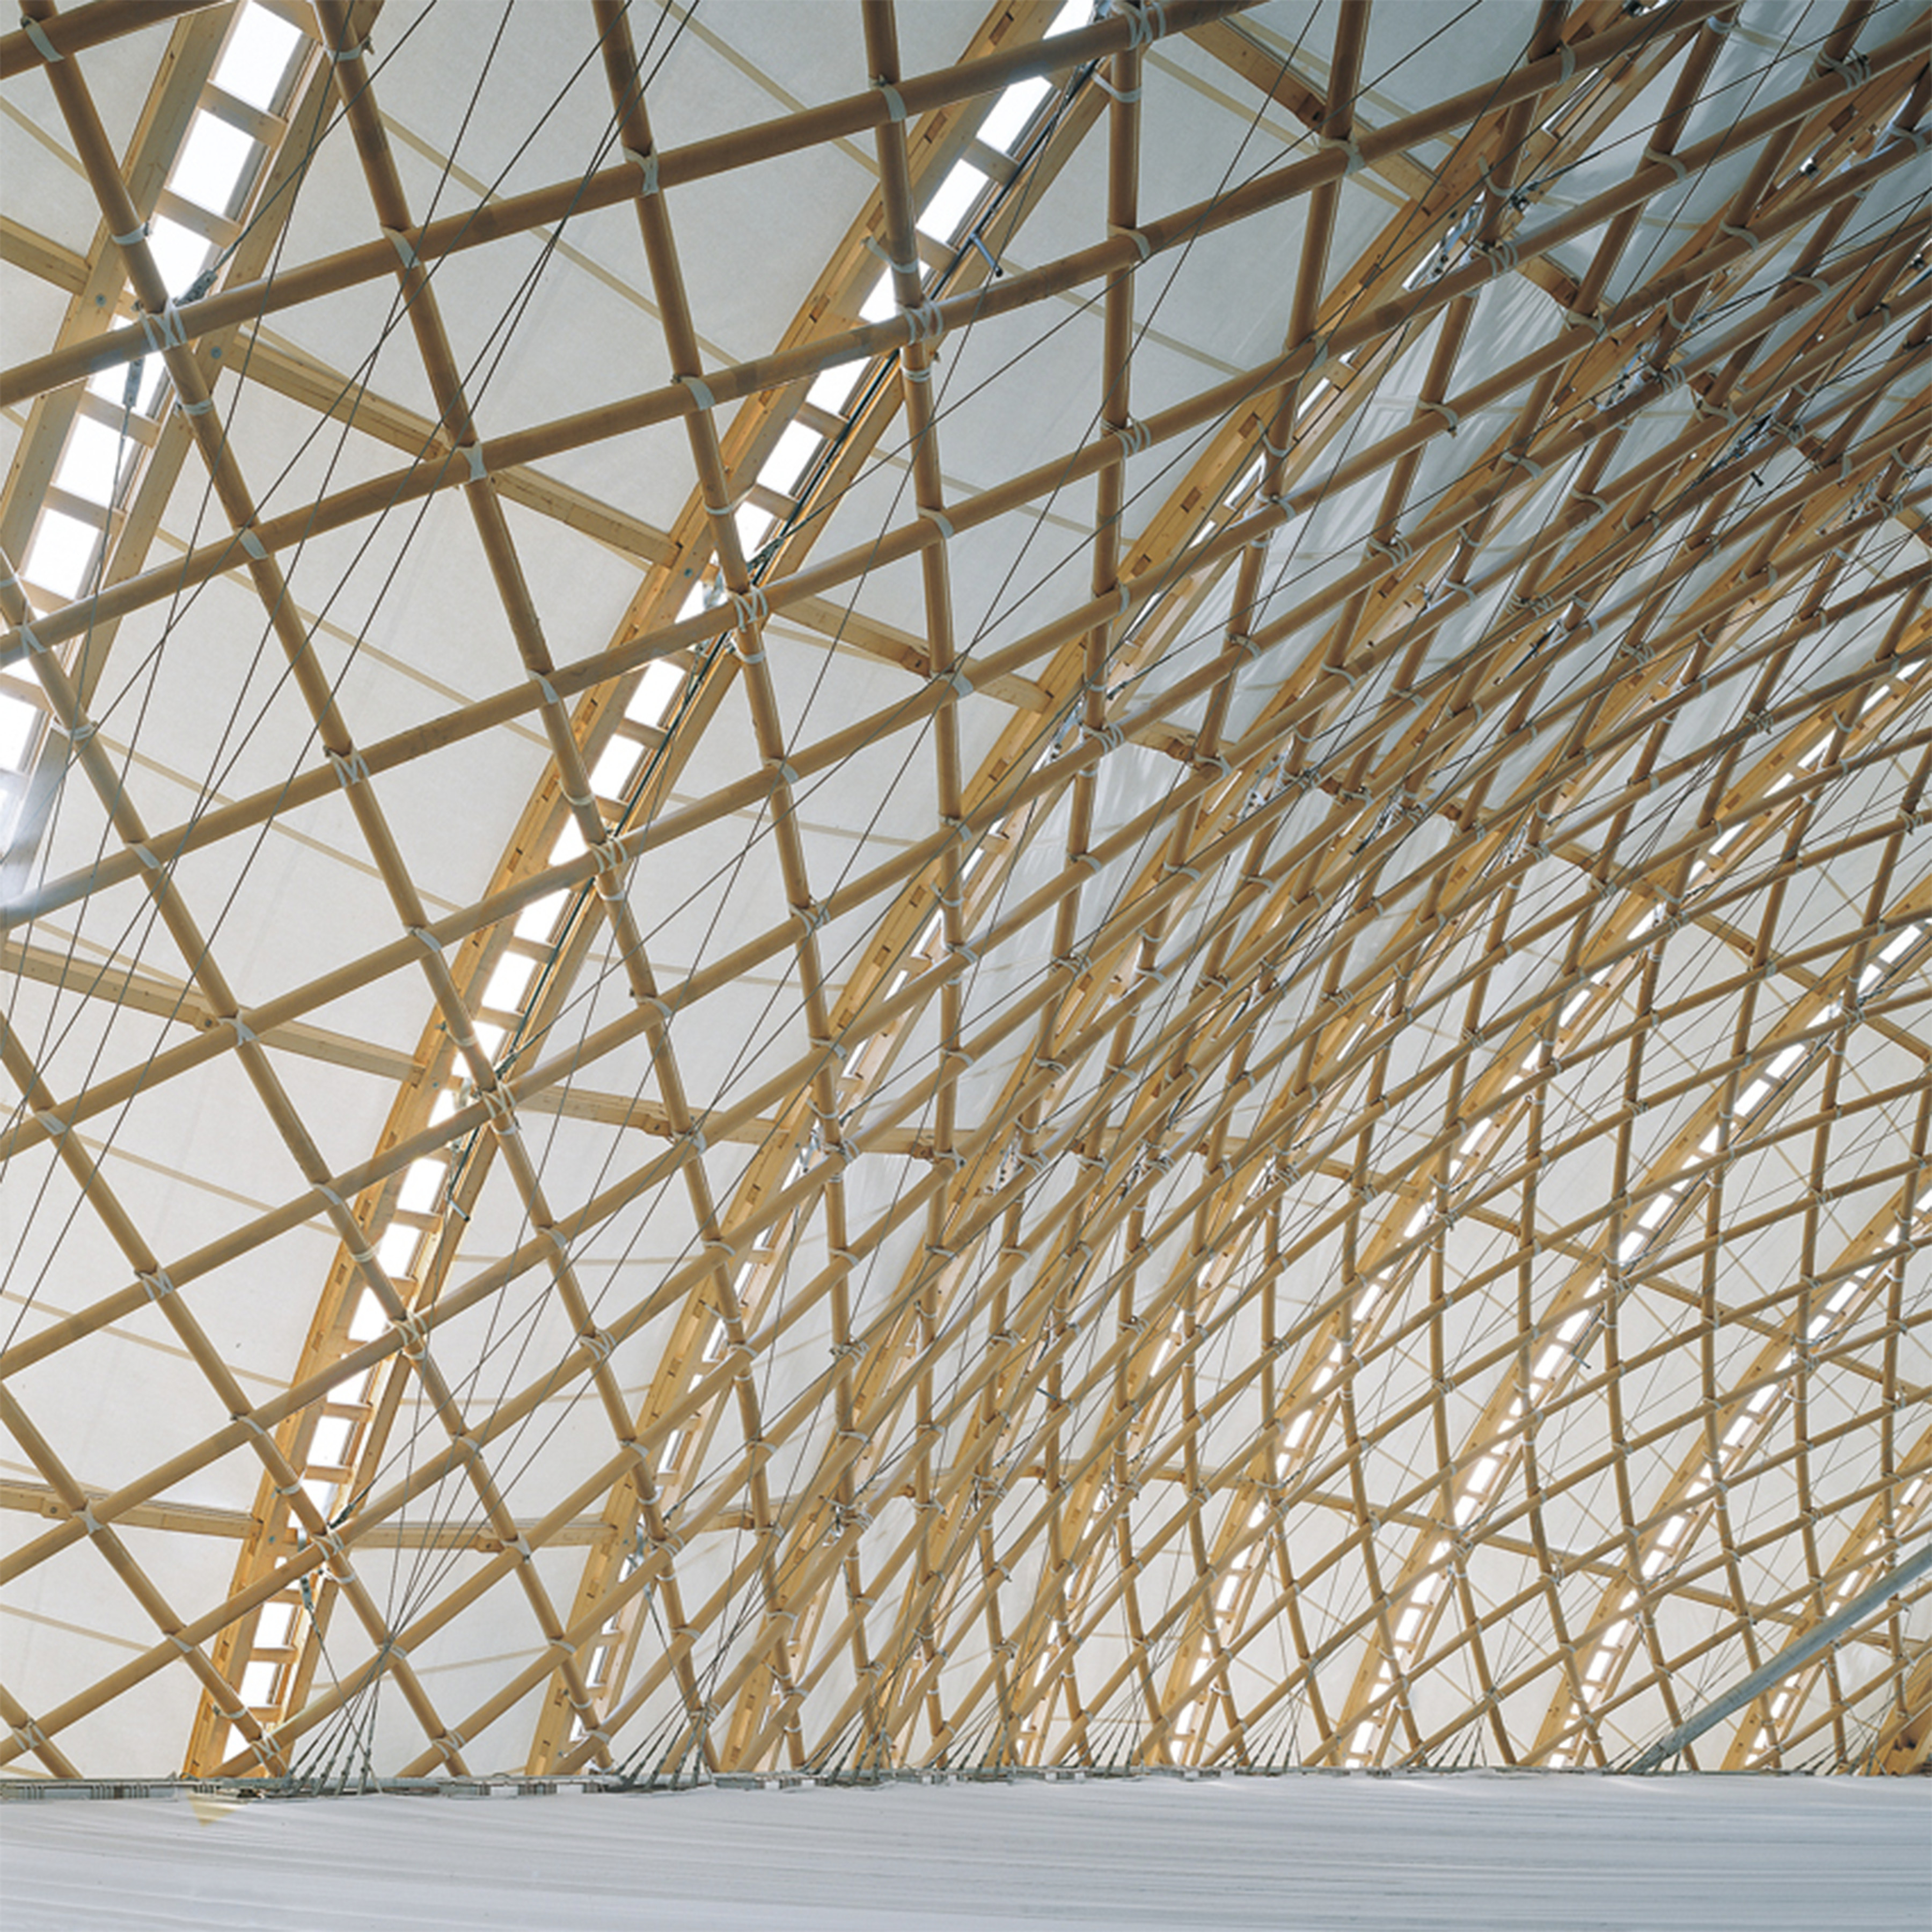
\includegraphics[width=0.32\MediaWidth]{hannover_int.jpg}\label{fig:hannover_a}}
%		\hspace*{\fill}
%		\subfloat[][Sky view]{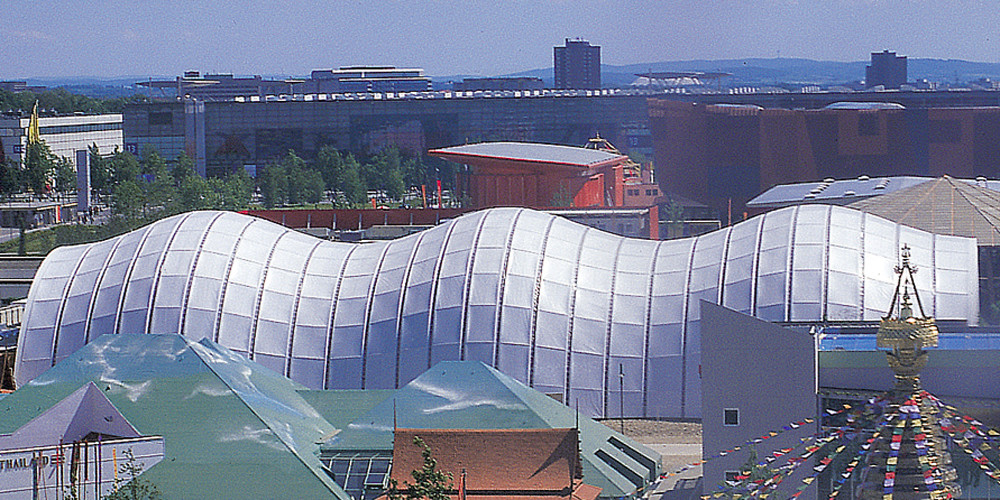
\includegraphics[width=0.64\MediaWidth]{hannover_sky.jpg}\label{fig:hannover_b}}
%%		\hrule
%		\captionof{figure}[Cardboard gridshell built in 2000 in Hannover, Germany]{Cardboard gridshell built in 2000 in Hannover, Germany.}\label{fig:hannover}
%		\hrule
%		\subfloat[][Interior view]{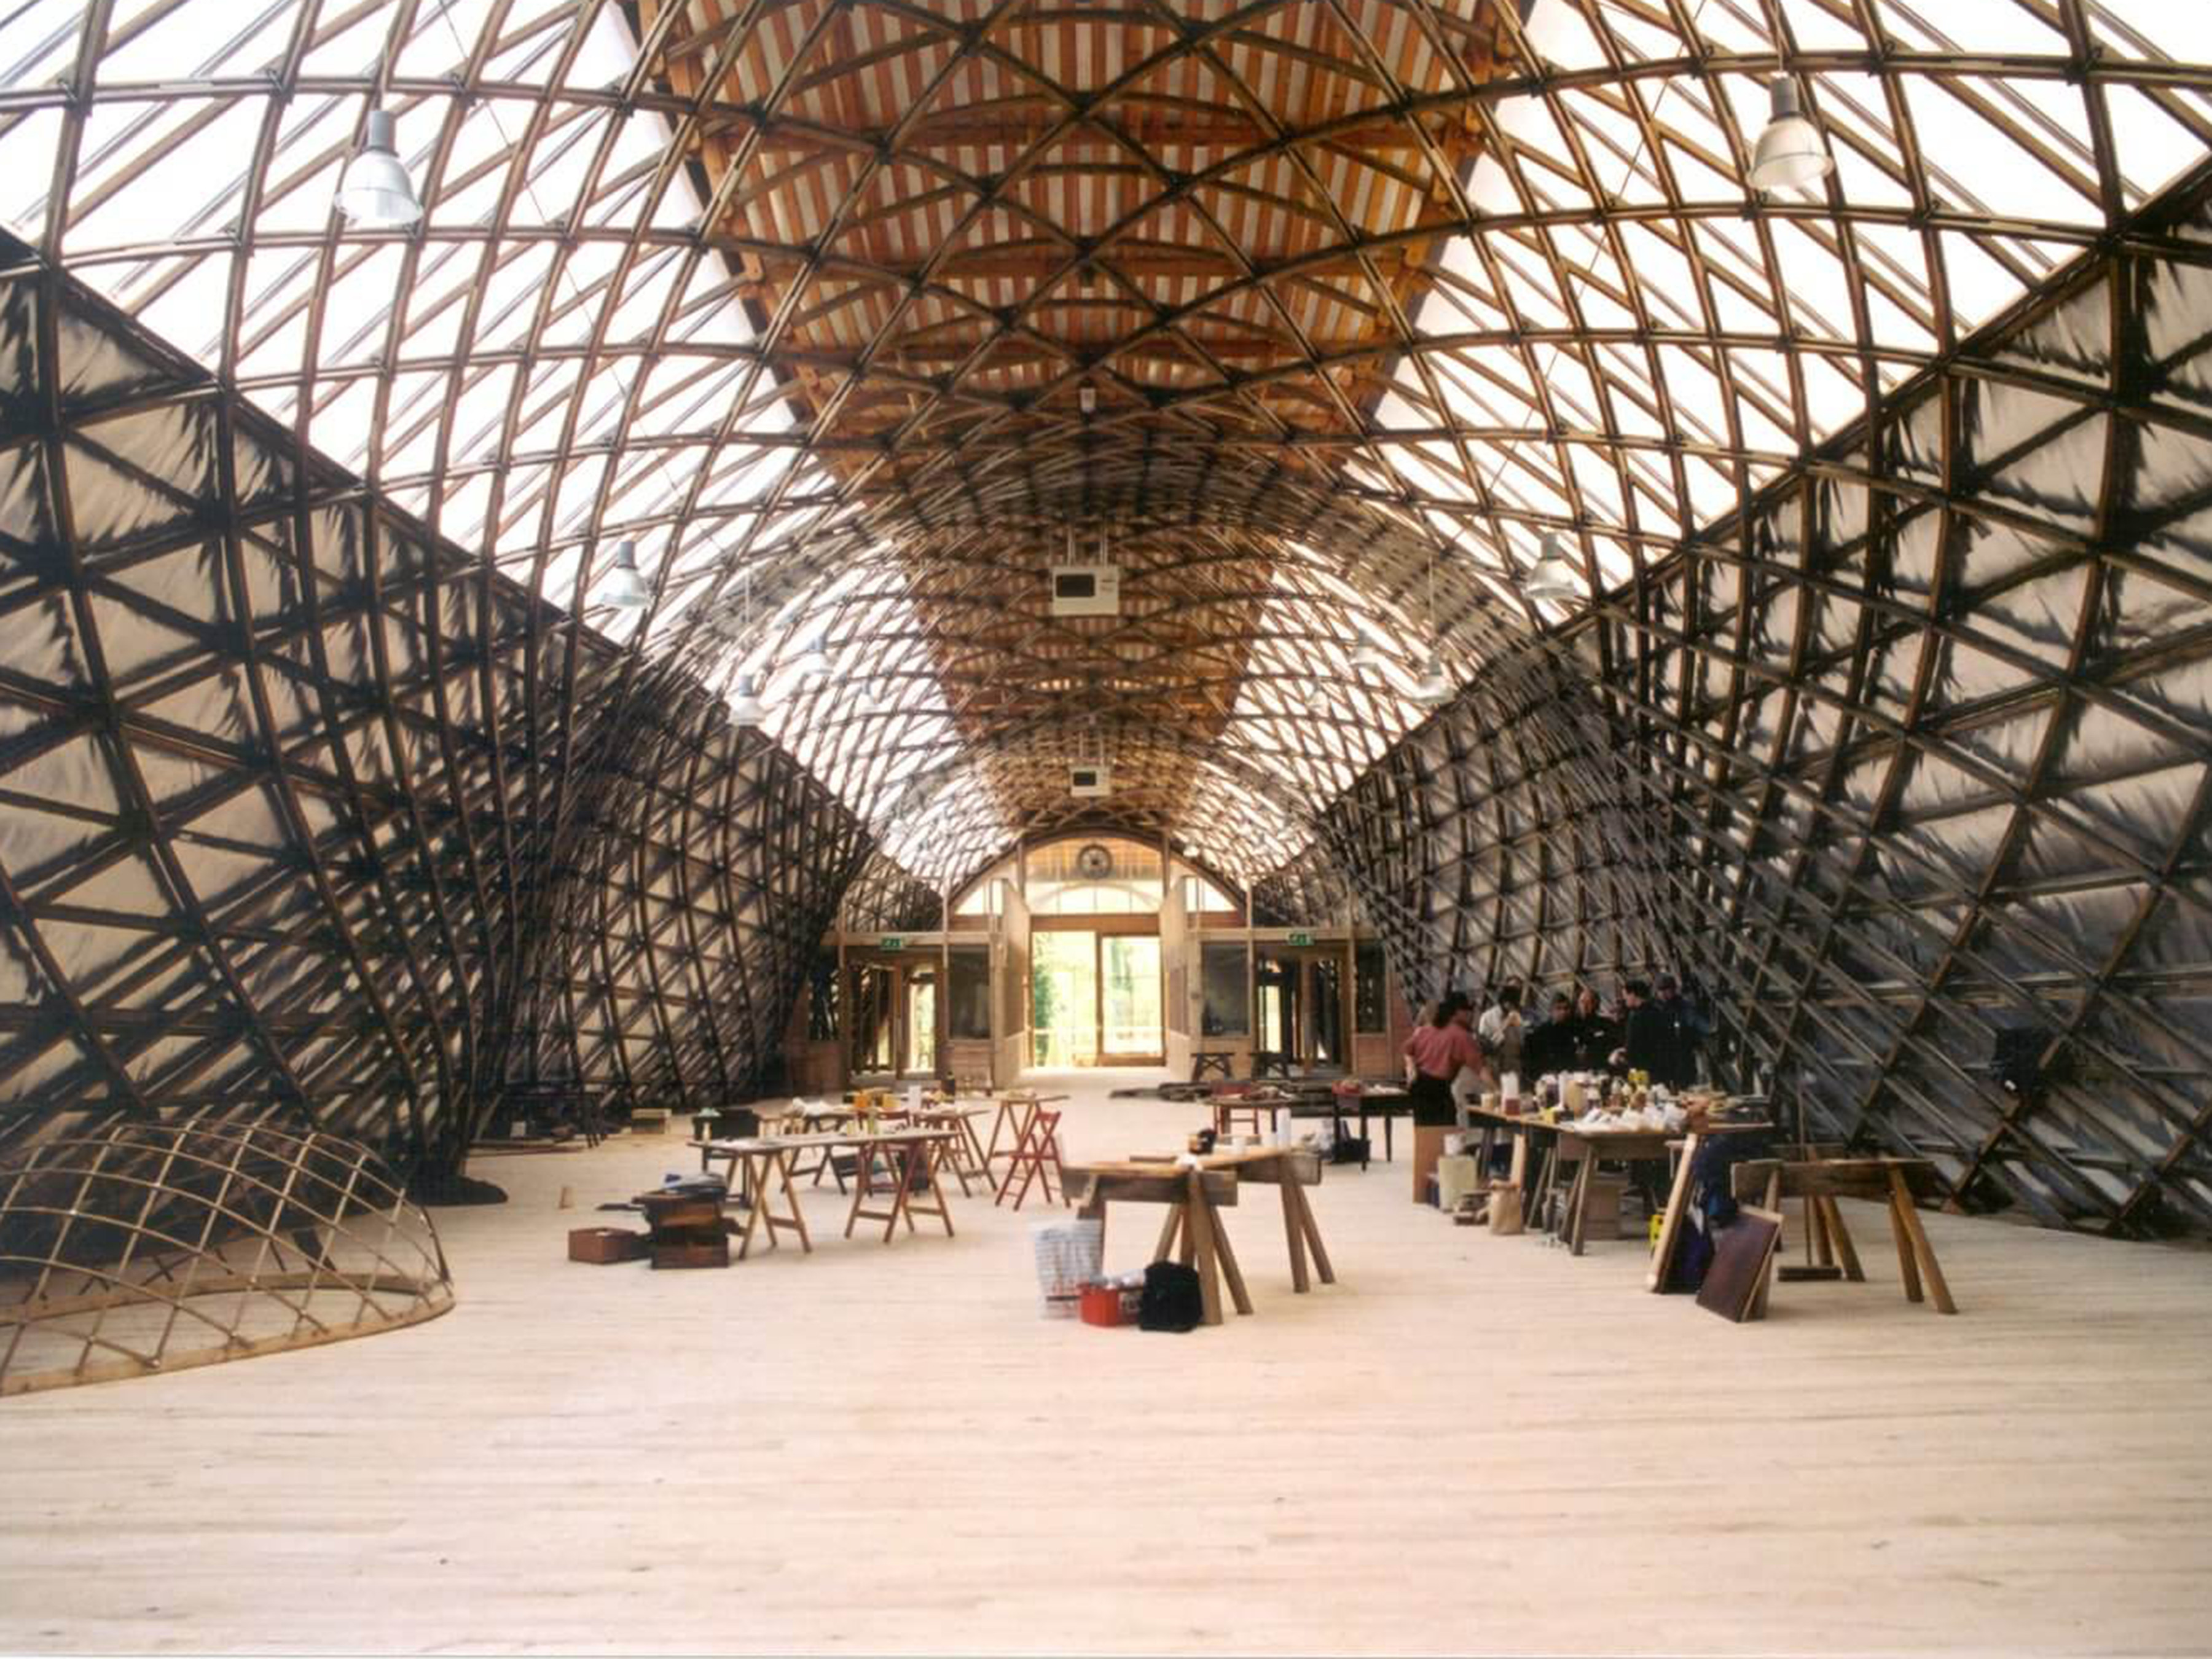
\includegraphics[width=0.48\MediaWidth]{downland_b.jpg}\label{fig:downland_a}}
%		\hspace*{\fill}
%		\subfloat[][Exterior view]{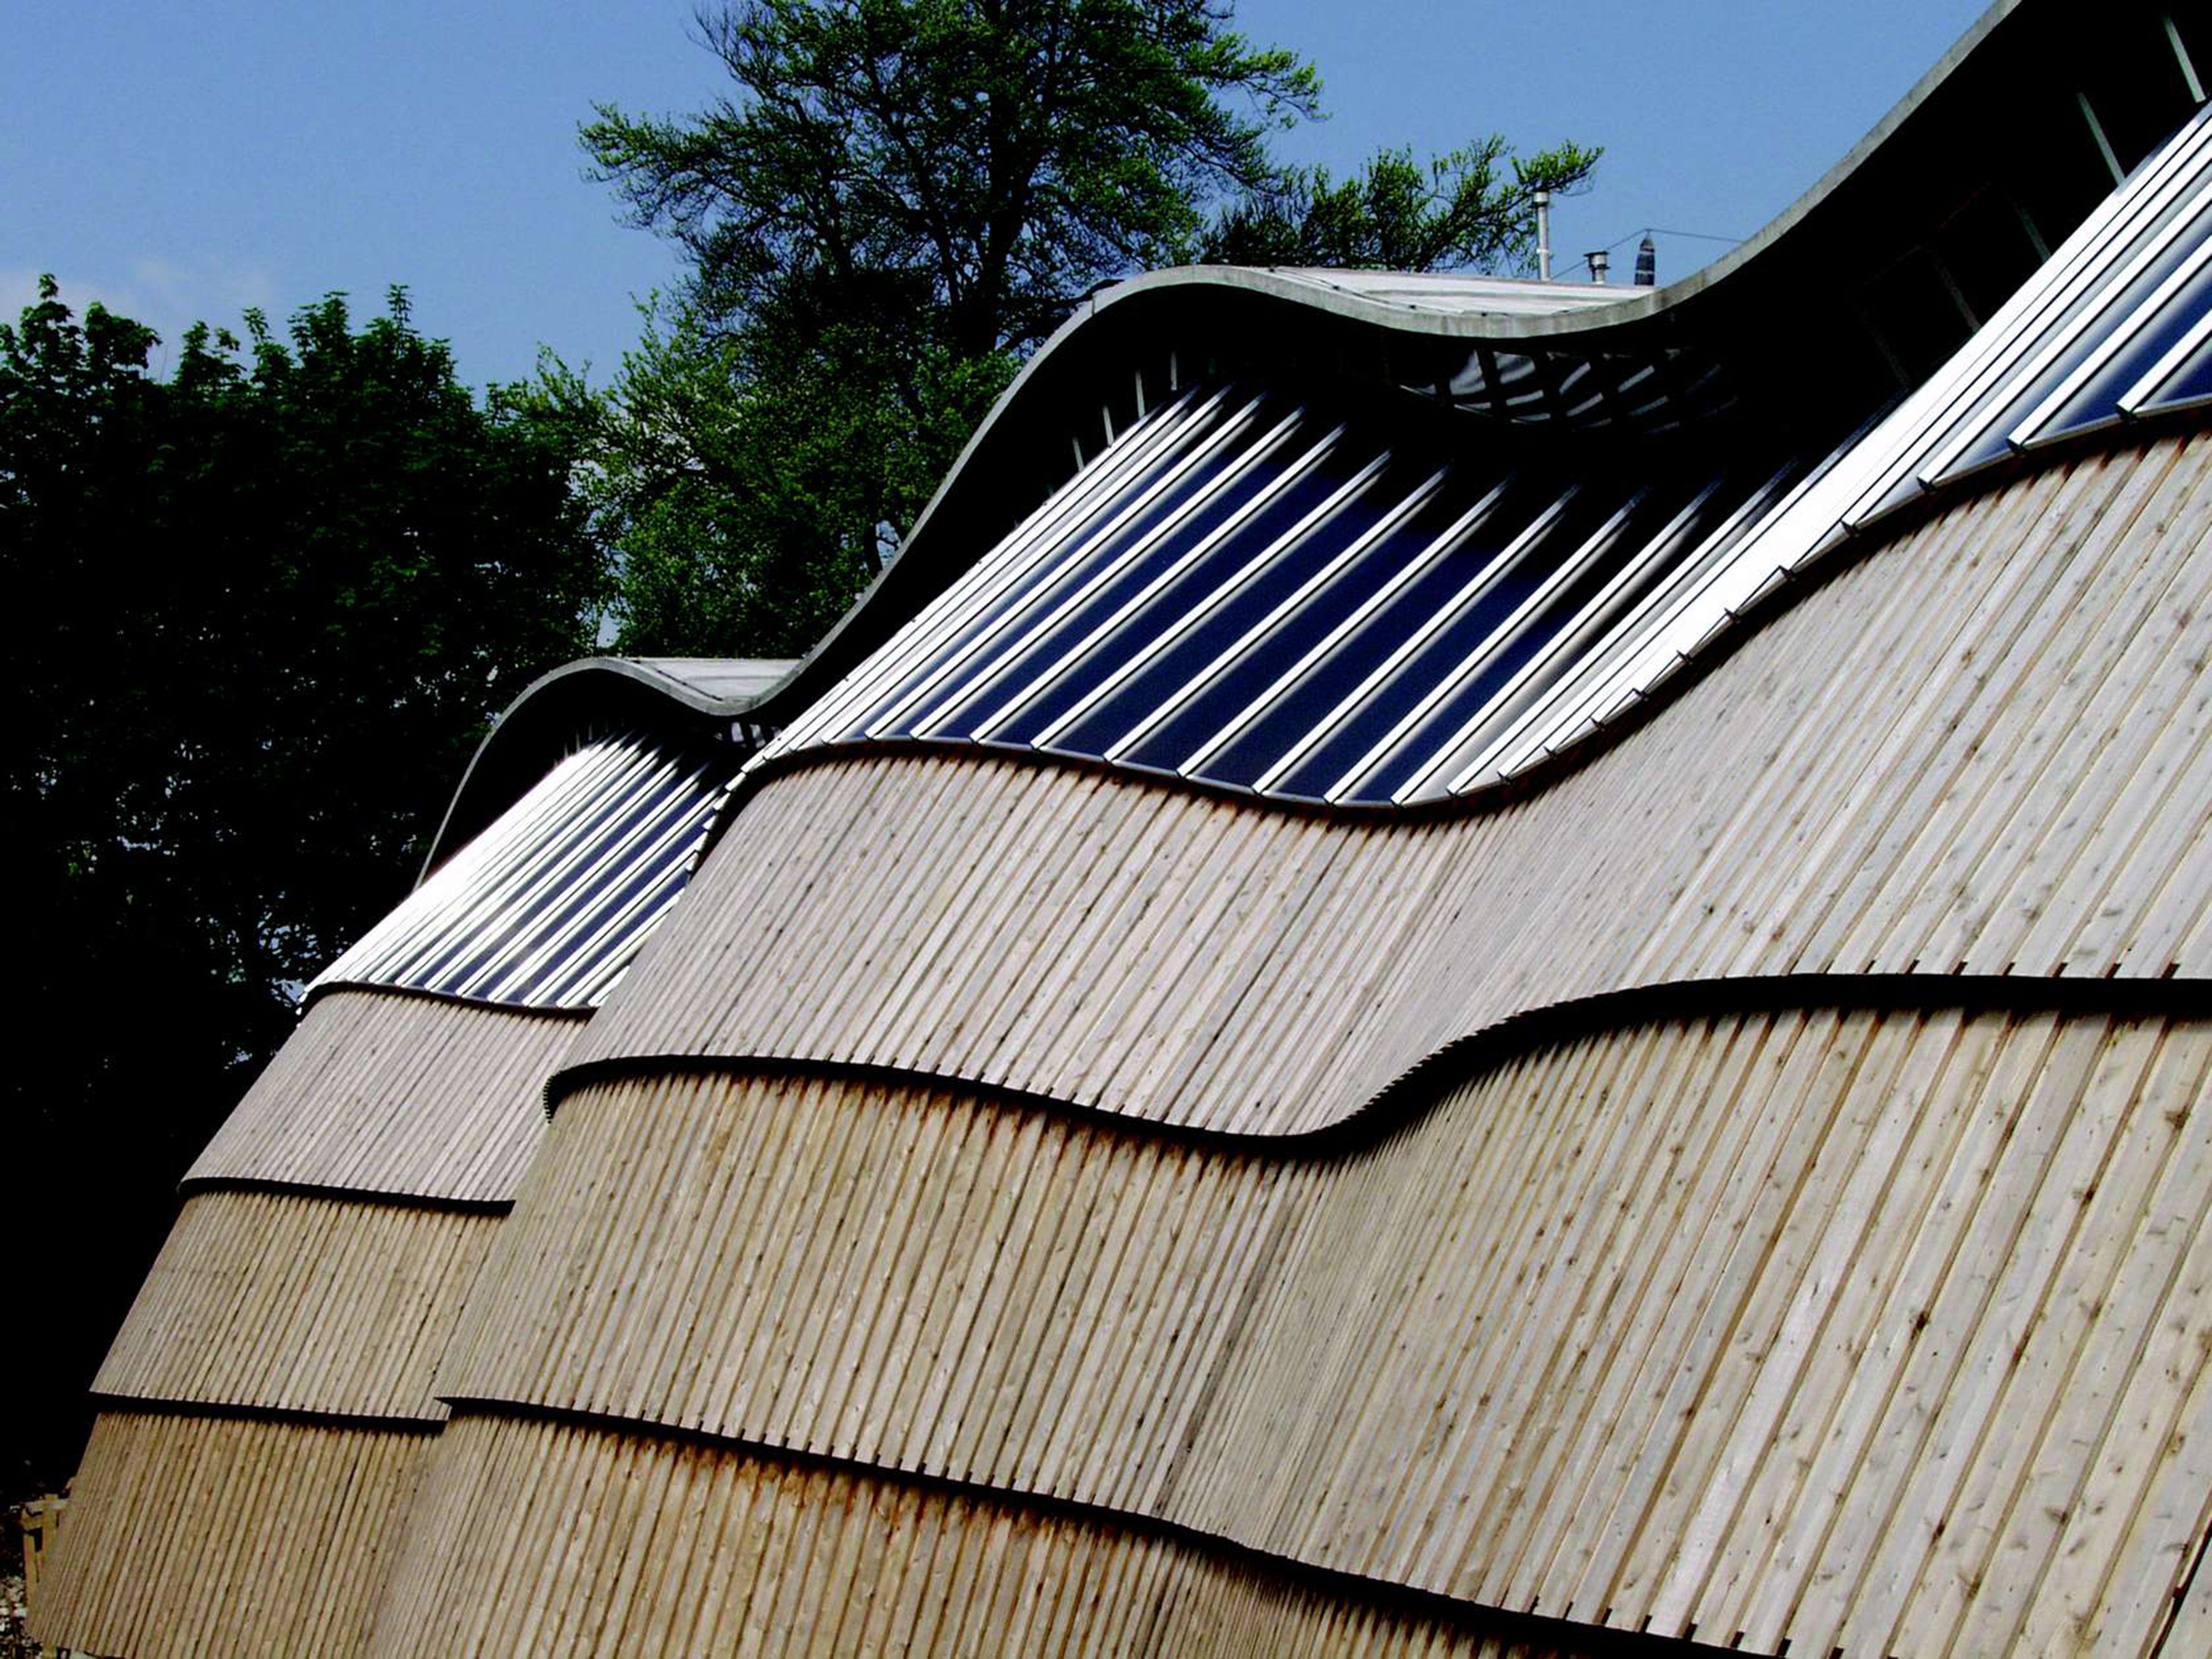
\includegraphics[width=0.48\MediaWidth]{downland_a.jpg}\label{fig:downland_b}}
%		\hrule
%		\captionof{figure}[Timber gridshell built in 2002 in Downland, England]{Timber gridshell built in 2002 in Downland, England.}\label{fig:downland}
%		\hrule
%%	\end{fullpage}
%\end{figure}

%\clearpage
%\begin{figure}[t]
%		\hrule
%		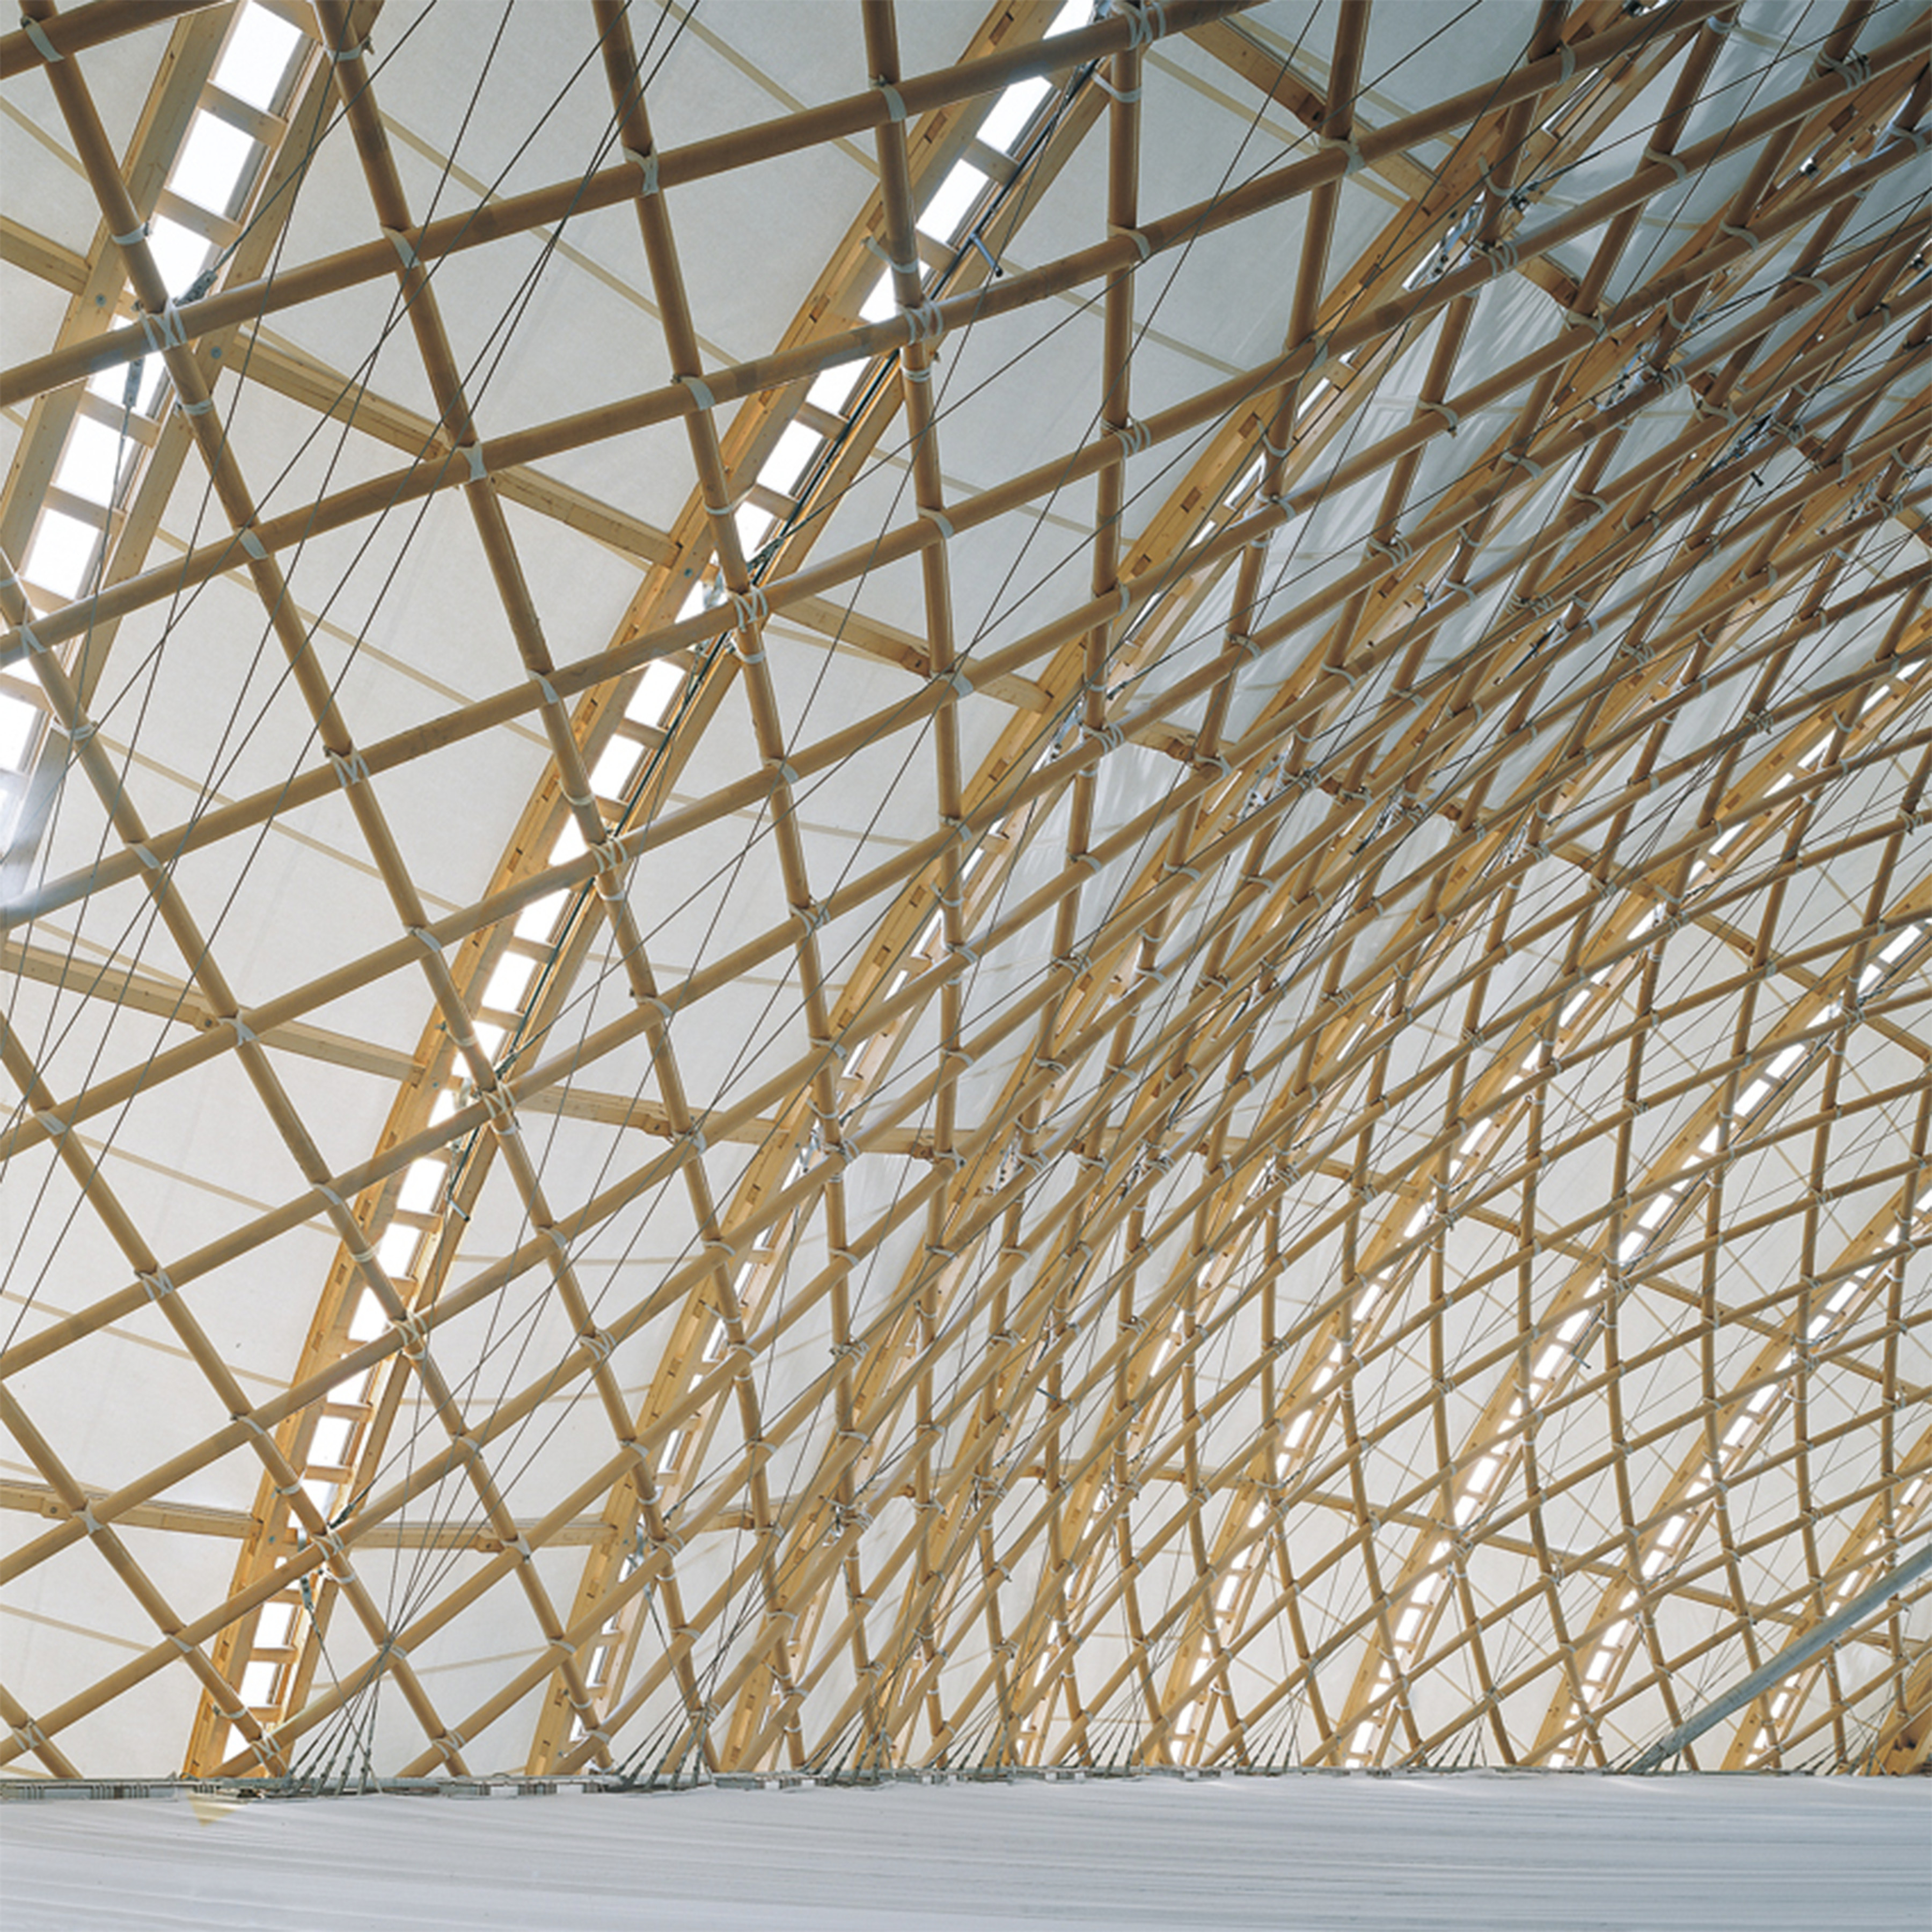
\includegraphics[width=0.32\MediaWidth]{hannover_int.jpg}
%		\hspace*{\fill}
%		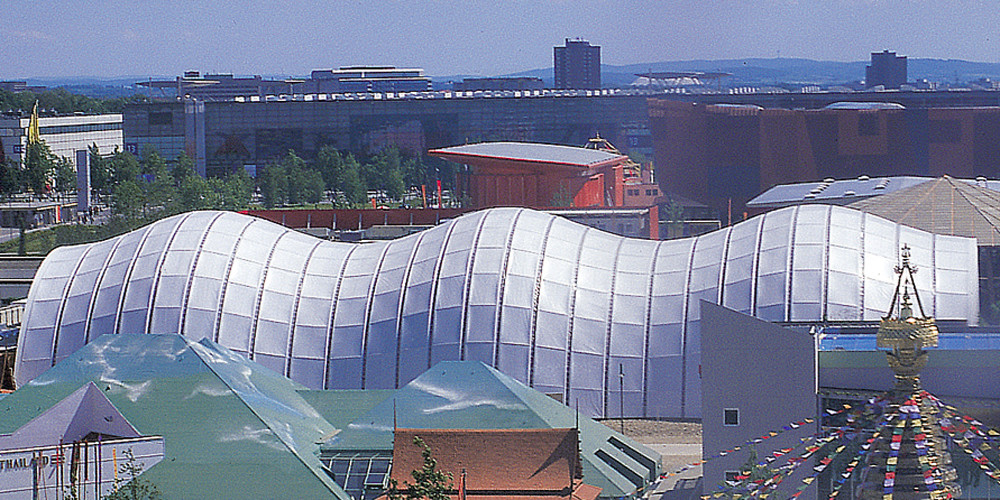
\includegraphics[width=0.64\MediaWidth]{hannover_sky.jpg}\label{fig:hannover_b}
%		\hrule
%		\captionof{figure}[Cardboard gridshell built in 2000 in Hannover, Germany]{Cardboard gridshell built in 2000 in Hannover, Germany.}
%		\hrule
%\end{figure}

%https://tex.stackexchange.com/questions/122314/figures-what-is-the-difference-between-using-subfig-or-subfigure/122329

\captionsetup{subrefformat=parens}

\begin{figure}[t]
\hrule
	\begin{subfigure}[b]{0.32\MediaWidth}
		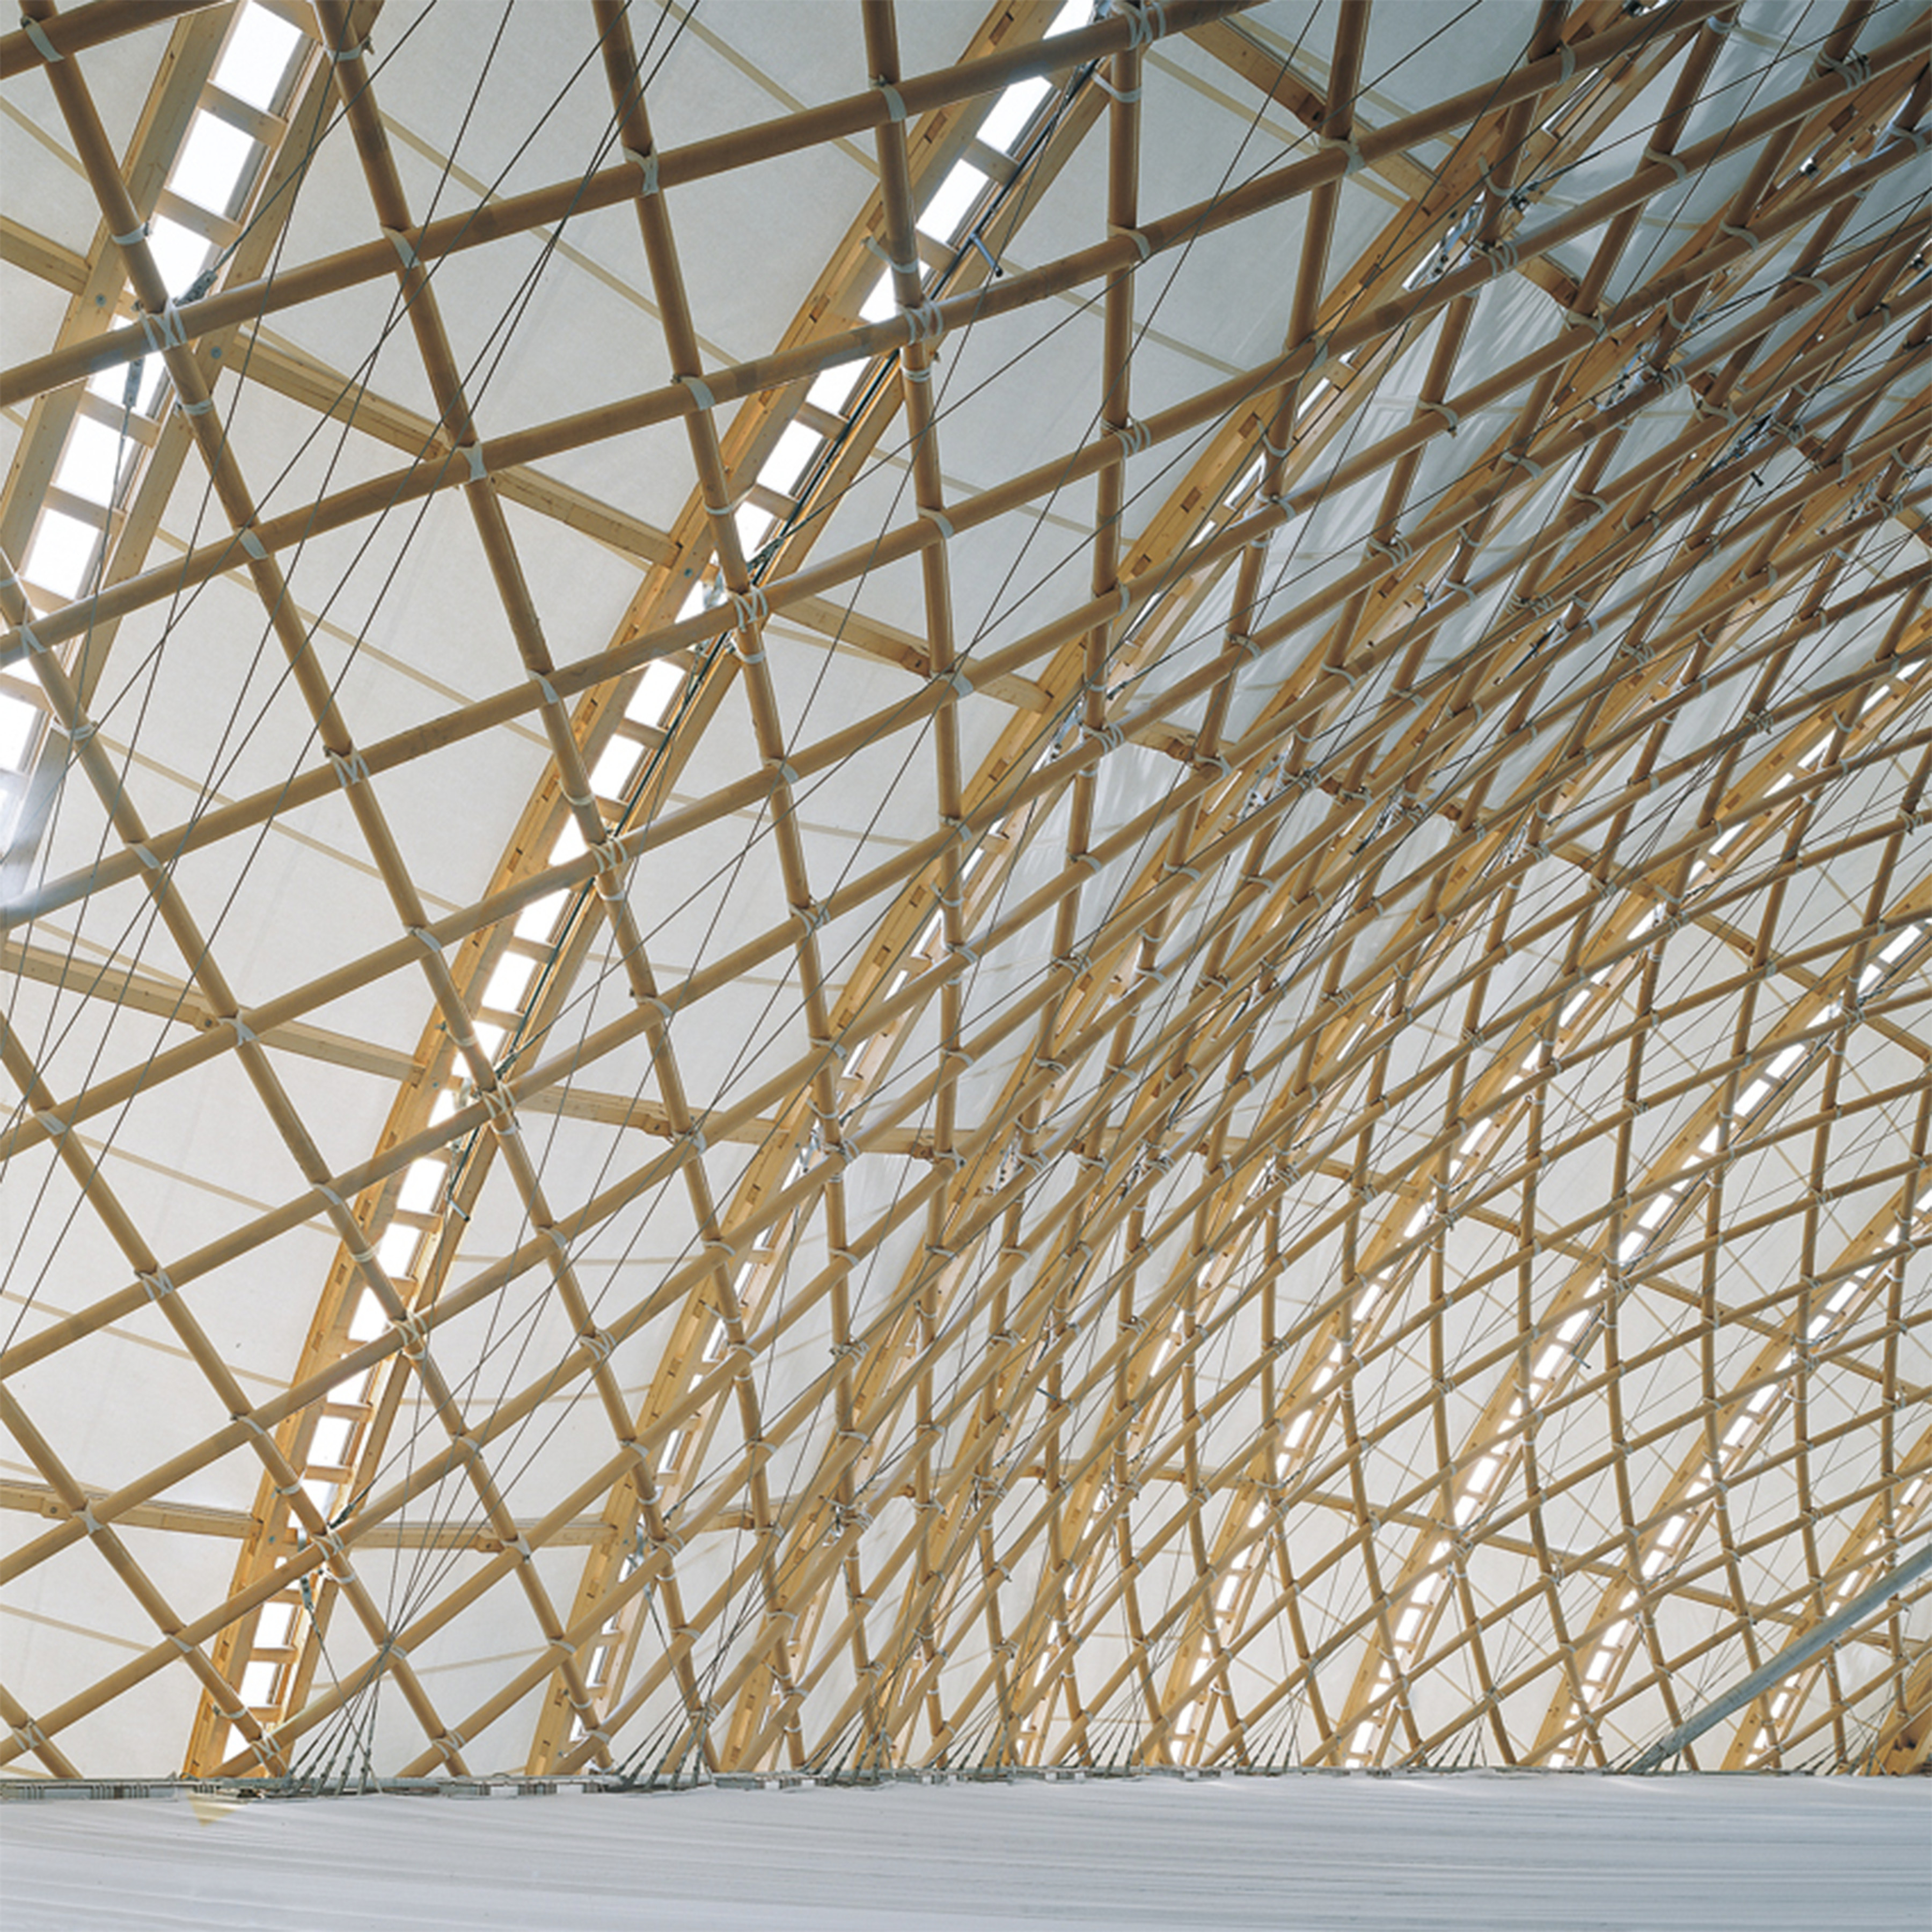
\includegraphics[width=\textwidth]{hannover_int.jpg}
		\caption{my first sub caption}
		\label{fig:hannover_a}
	\end{subfigure}
\hspace{\fill}%
	\begin{subfigure}[b]{0.64\MediaWidth}
		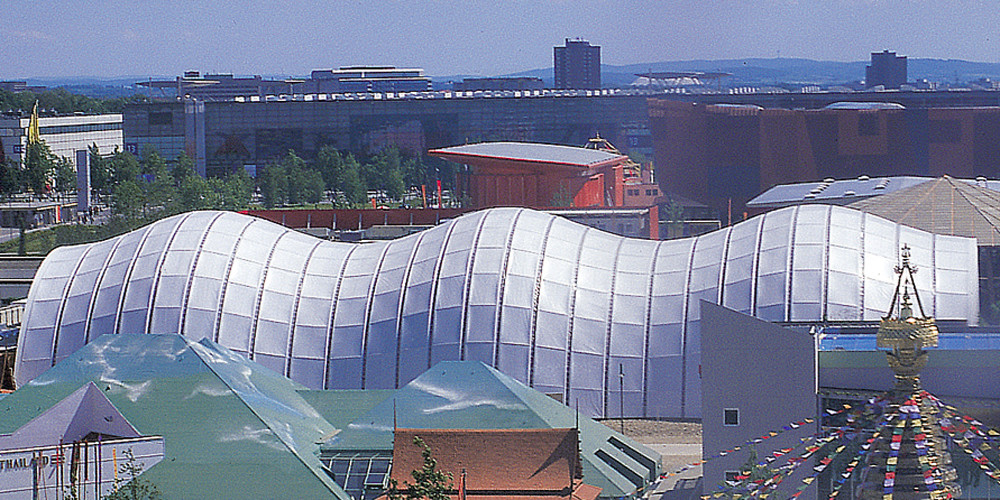
\includegraphics[width=\textwidth]{hannover_sky.jpg}
		\caption{my second sub caption}
		\label{fig:hannover_b}
	\end{subfigure}
\caption{Cardboard gridshell built in 2000 in Hannover, Germany.}
\label{fig:hannover}
\hrule
\end{figure}

smldksmldk

Main \cref{fig:hannover}, A \ref{fig:hannover_a}, B \ref{fig:hannover_b} 



The grid pitch is \SI{1.0}{m} except in weaker areas where it is \SI{0.5}{m}. There, the grid is twice denser to achieve the required buckling resistance \cite{Harris2003}. Rib-lath bracing was preferred to steel cable bracing as ribs were deemed to offer a more convenient support for the cladding and to reduce the complexity of the connection. A new connection system was developed to avoid the cost of drilling thousands of slotted holes that would, in addition, reduce the cross-section area, while maintaining the required scissor behaviour for the deformation of the timber lattice.\footnote{This detail was \href{https://patents.google.com/patent/GB2361504A/en?q=\%22A+coupling+and+a+method+of+constructing+grid+shell+buildings+using+such+a+coupling\%22&country=GB}{patented} by the design team and the client.}

The flat lattice was laid out on a scaffold platform. Unlike the Japan Pavilion, the lattice was progressively lowered down into position. This stage took 6 weeks. Once deformed, the shear blocks were introduced in the grid and bracing rib-laths were installed, giving its full strength to the shell. Finally the gridshell was cladded with a mix of polycarbonate plates (to let the light in) and timber boards on top of insulation panels and a rain screen.

It is worthwhile to mention that for the first time the form was not found by inverting some sort of hanging chain model that would produce a pure funicular shape where only compression occurred. Instead, the shape was the result of a numerical computation that took into account the bending behaviour of the laths.\footnote{This software was developed under the supervision of Chris Williams of the university of Bath.} \citet{Harris2003} argued that computer models enabled some interactivity in the form-finding process that would not be possible with physical models, leading to a better synergy between architectural and structural requirements. They also argued that physical models contributed invaluably to the development of a creative and efficient design throughout the project.

\subsubsection{Lothian Gridshell, Pishwanton, Scotland, 2002}
This project deserves some attention because the developed approach was completely different from the projects exposed until now~: \blockcquote[]{Lowenstein2002}{Previous projects have portrayed the method as a highly technical use of a low-tech resources. This, however, needs not be the case as we see with this project \belp{}}. The structure was the result of \blockcquote[]{bdonline2002}{\belp{} an unusual collaboration between sole practitioner Christopher Day, engineer David Tasker, a crowd of local volunteers and (more unusually) the philosophies of Rudolf Steiner and Johann Wolfgang Goethe}.\footnote{From the online paper \textquote{The other gridshell} : \url{http://www.bdonline.co.uk/the-other-gridshell/1020435.article}}

The single-layer gridshell was made out of local larch. Once erected by hands, the dome-like shape covered about \SI{80}{m^2} and spanned 10 meters. The grid was braced with timber boards (see \cref{fig:pishwanton_a}) and covered with a planted turf roof (see \cref{fig:pishwanton_b}). Some calculations were made but in the end, it had to carry load testing to prove its safety and gain its regulation approval.\footnote{\blockcquote[]{bdonline2002}{There were a lot of calculations but no computer-generated models to show they all added up. In fact, the form was previously established with scale models. When it came to gaining Building Regulations approval, the team needed to prove that the building would be strong enough. So Tasker arranged for the unfinished structure to be loaded with about 18 tonnes of sand from a local quarry – equivalent to the maximum predicted snow load, plus a safety factor.}}

\subsubsection{Woodland Centre, Filmwell, England, 2003}
The gridshell of the Woodland Centre was built 7 years after the project had started (see \cref{fig:flimwell_a}).\footnote{More to be found at : \href{http://www.fourthdoor.org/annular/?page_id=441}{Growing and making Flimwell’s chestnut gridshell}.} The building was designed by architect Feilden Clegg and engineers from Atelier One. It was part of a larger research and development project that aimed at developing chestnut -- a low grad wood -- as a construction material.\footnote{This projet was conducted by the \href{http://www.bre.co.uk/}{Building Research Establishment}.}

The building, still existing, is composed of 5 barrel vaults spanning 12 meters and about 5 meters wide (see \cref{fig:flimwell_b}). It covers about \SI{300}{m^2} \cite{Lowenstein2004}. Each vault module is a transportable unit composed of two curved arches. A single layer gridshell was then applied to this primary frame and braced with chestnut panels. The grid was made of laths with~\SI{75}{mm} x \SI{25}{mm} rectangular cross-section, assembled with simple bolts. On top of that, insulation materials and a membrane as rainscreen \cite{FourthDoor2003}.

\begin{figure}[t]
	% (%) required at end of lines to prevent extra space
	\hrule
	%
	%
	\begin{subfigure}[b]{\TwoMediaWidth}
		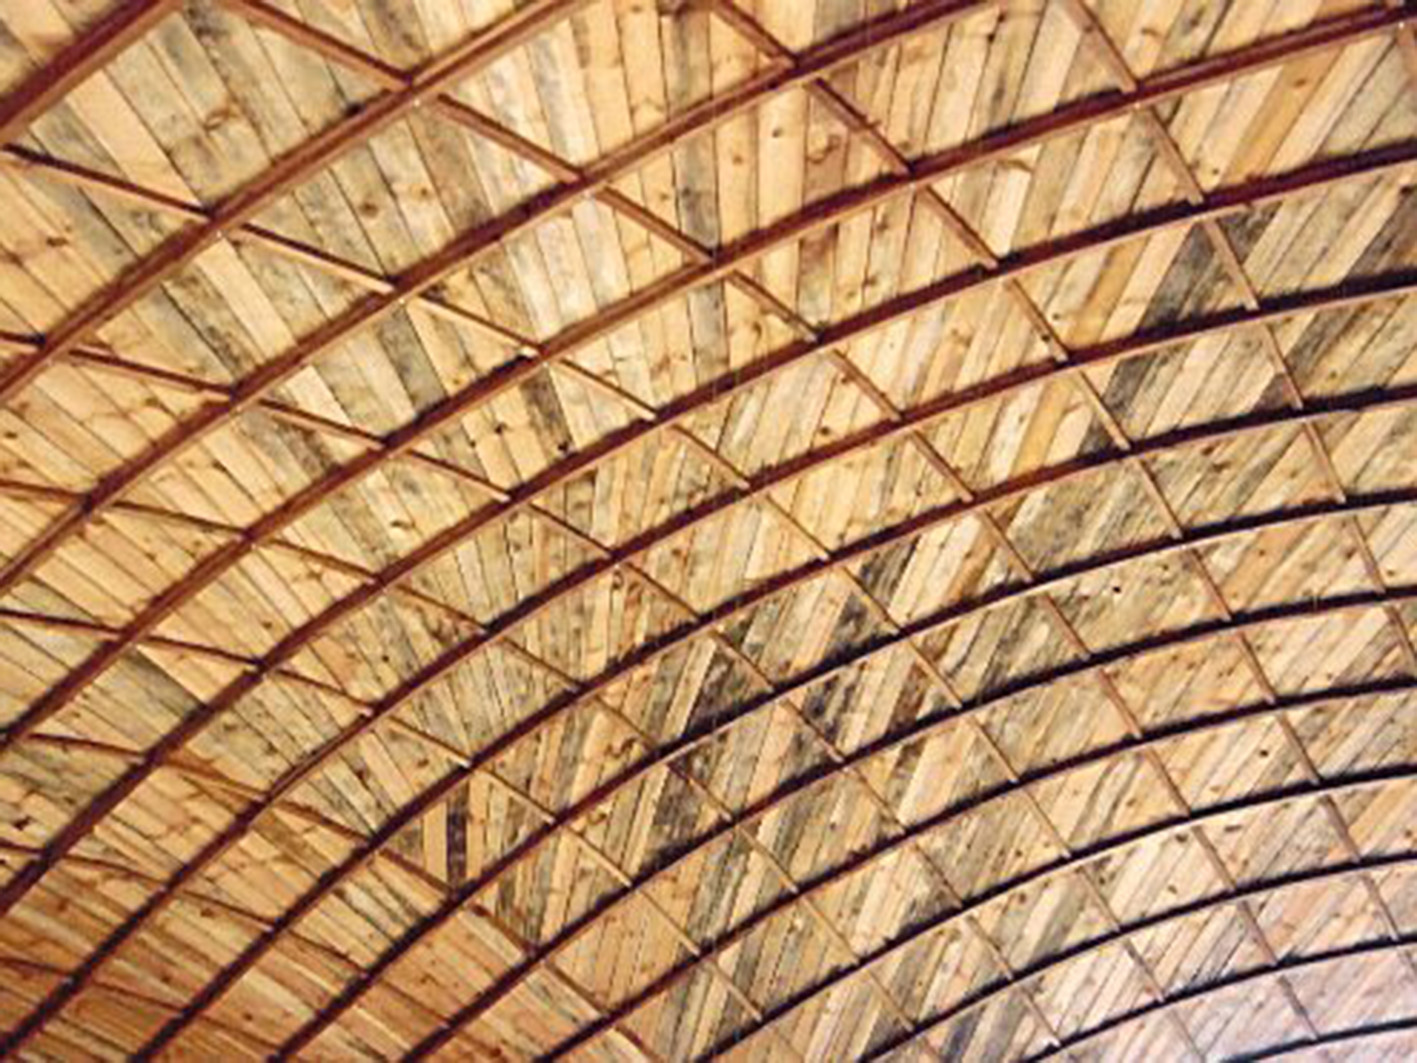
\includegraphics[width=\textwidth]{pishwanton_int.jpg}
		\caption{Interior view}
		\label{fig:pishwanton_a}
	\end{subfigure}%
	\hspace{\MediaGutterWidth}%
	\begin{subfigure}[b]{\TwoMediaWidth}
		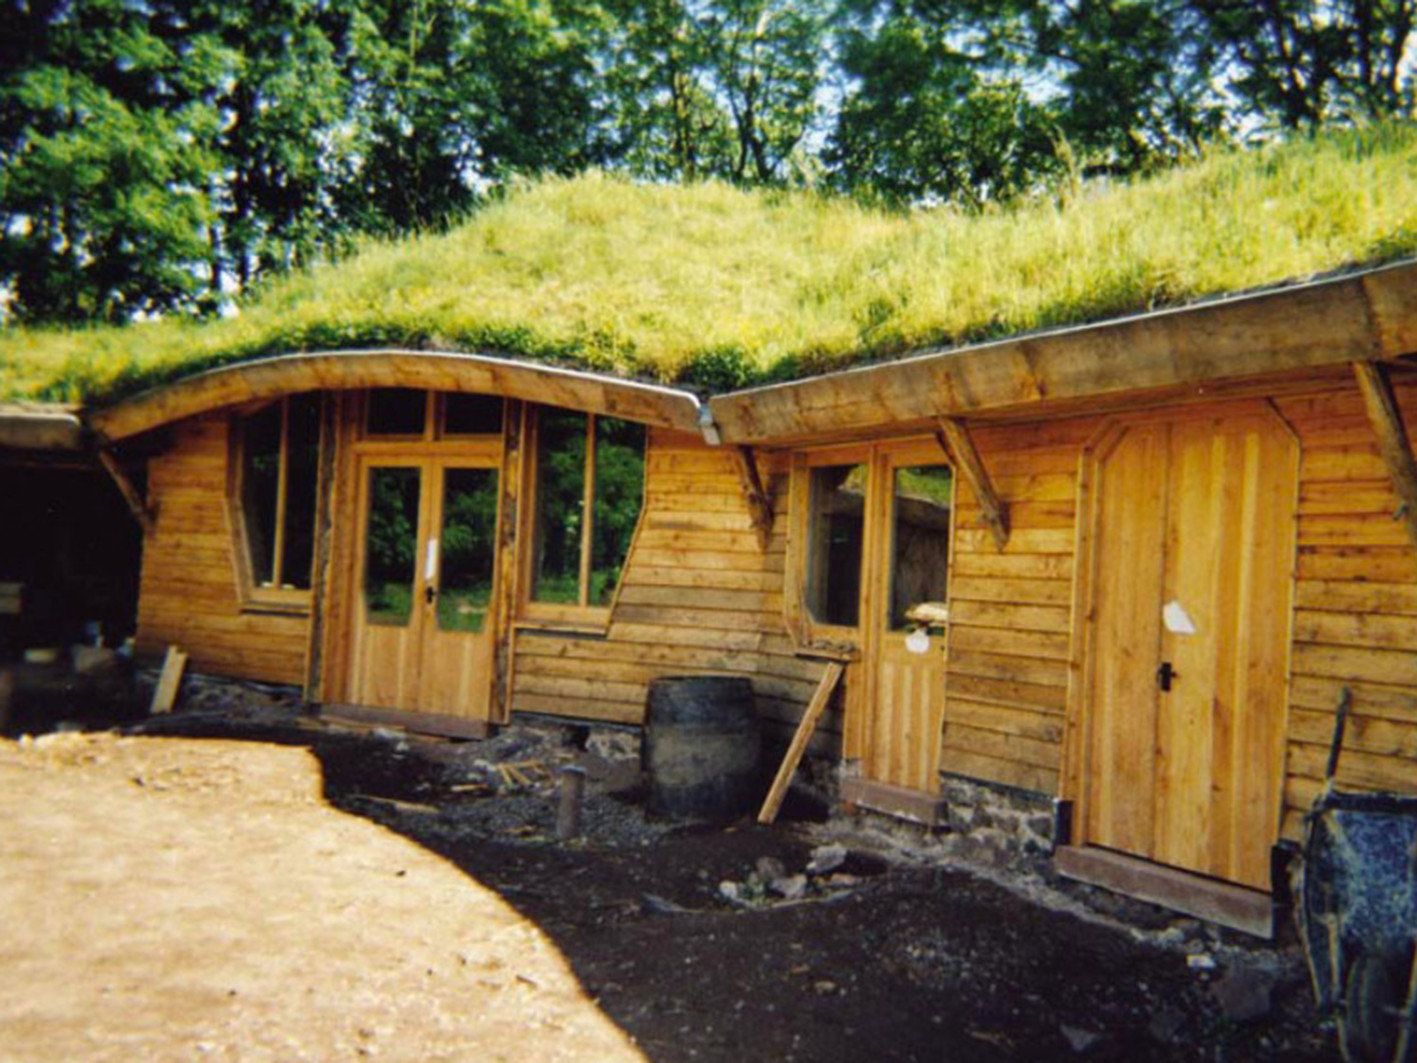
\includegraphics[width=\textwidth]{pishwanton_ext.jpg}
		\caption{Exterior view}
		\label{fig:pishwanton_b}
	\end{subfigure}
	\caption[Timber gridshell built in 2002 in Pishwanton, England]{Timber gridshell built in 2002 in Pishwanton, England.}
	\label{fig:pishwanton}
	%
	\subfigskip
	%
	\begin{subfigure}[b]{\TwoMediaWidth}
		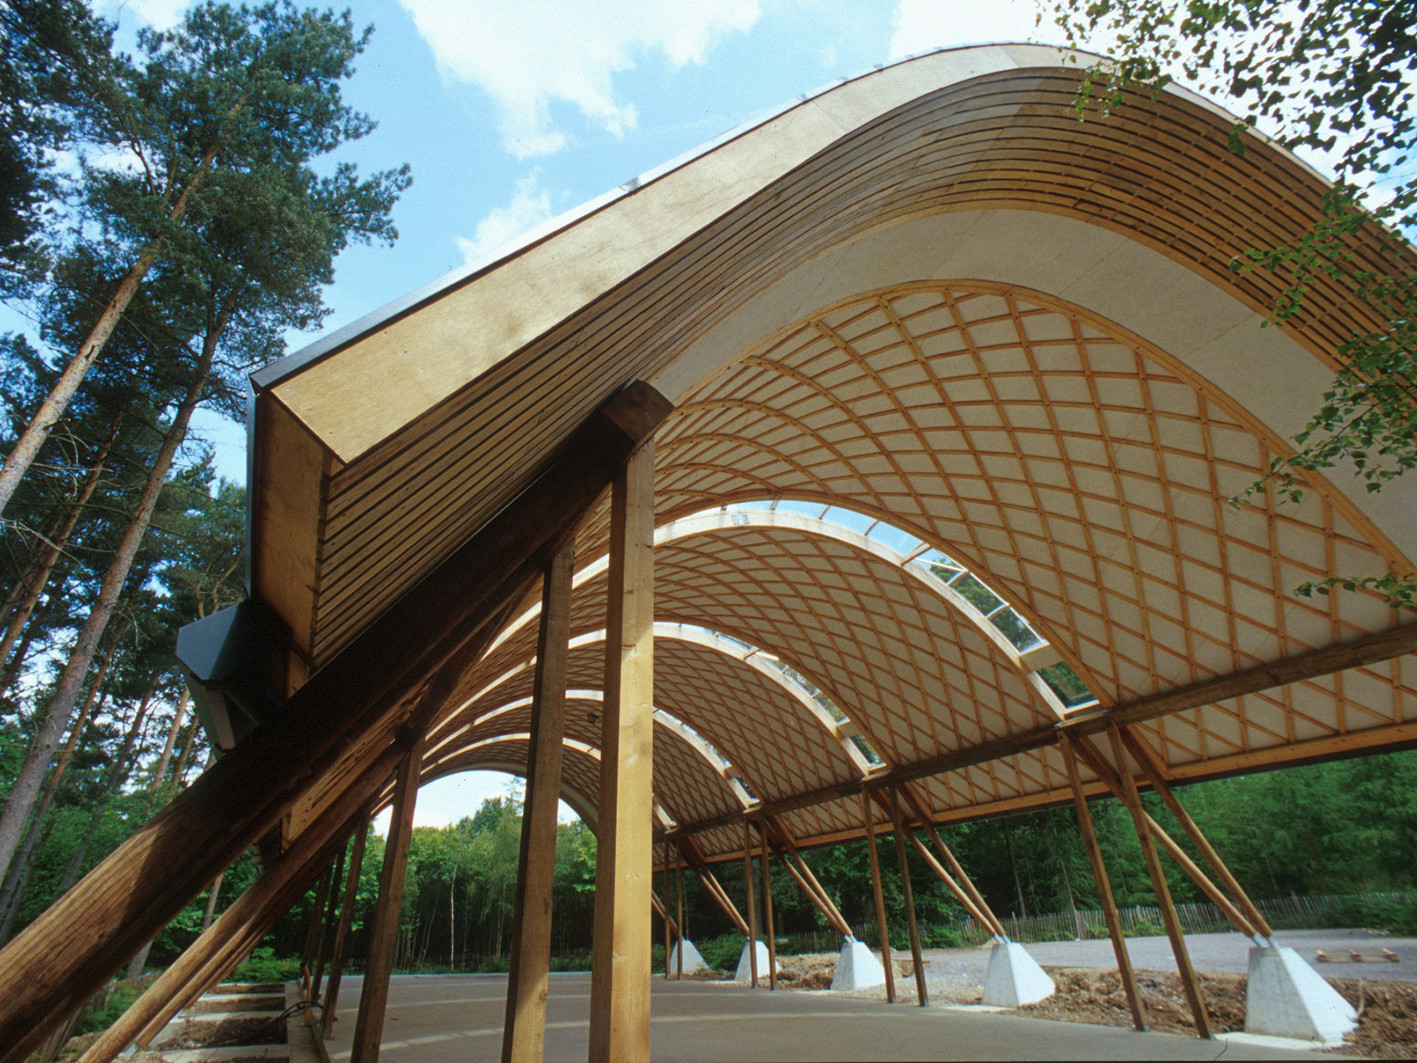
\includegraphics[width=\textwidth]{flimwell_int.jpg}
		\caption{Interior view}
		\label{fig:flimwell_a}
	\end{subfigure}%
	\hspace{\MediaGutterWidth}%
	\begin{subfigure}[b]{\TwoMediaWidth}
		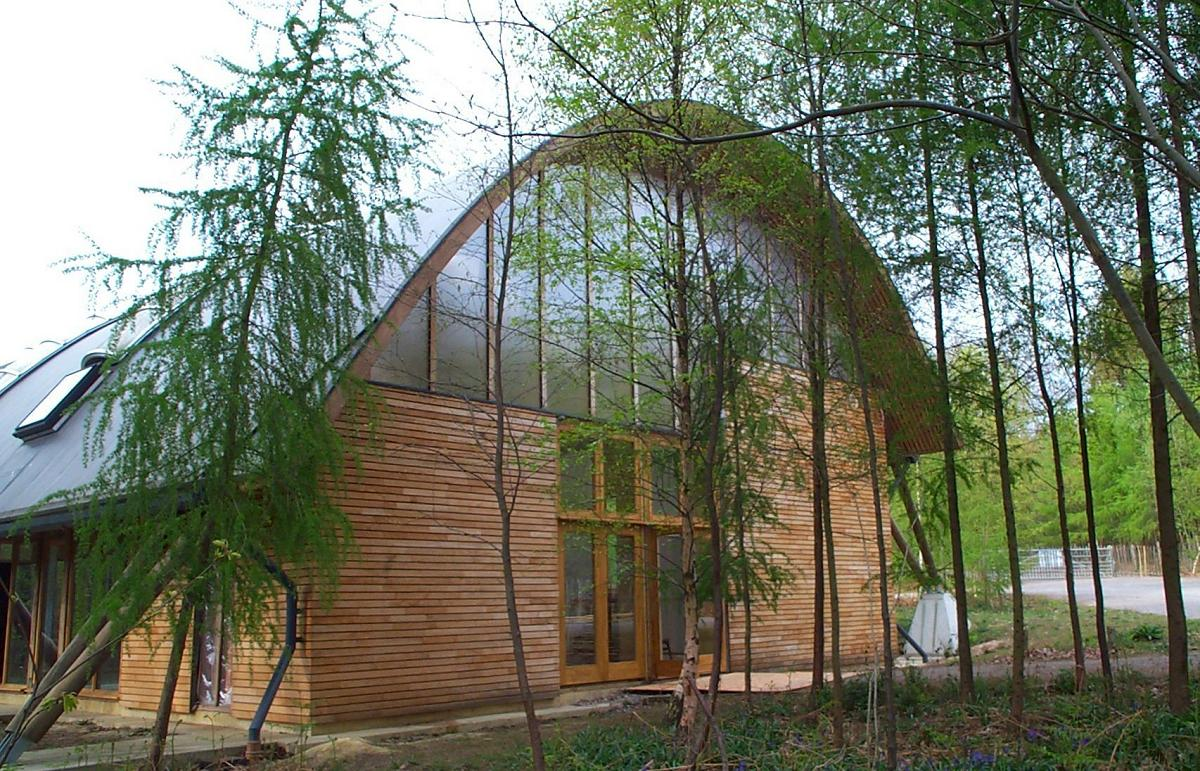
\includegraphics[width=\textwidth]{flimwell_ext.jpg}
		\caption{Exterior view}
		\label{fig:flimwell_b}
	\end{subfigure}
	\caption[Timber gridshell built in 2003 in Filmwell, England]{Timber gridshell built in 2003 in Filmwell, England.}
	\label{fig:flimwell}
	%
	\subfigskip
	%
	\begin{subfigure}[b]{\TwoMediaWidth}
		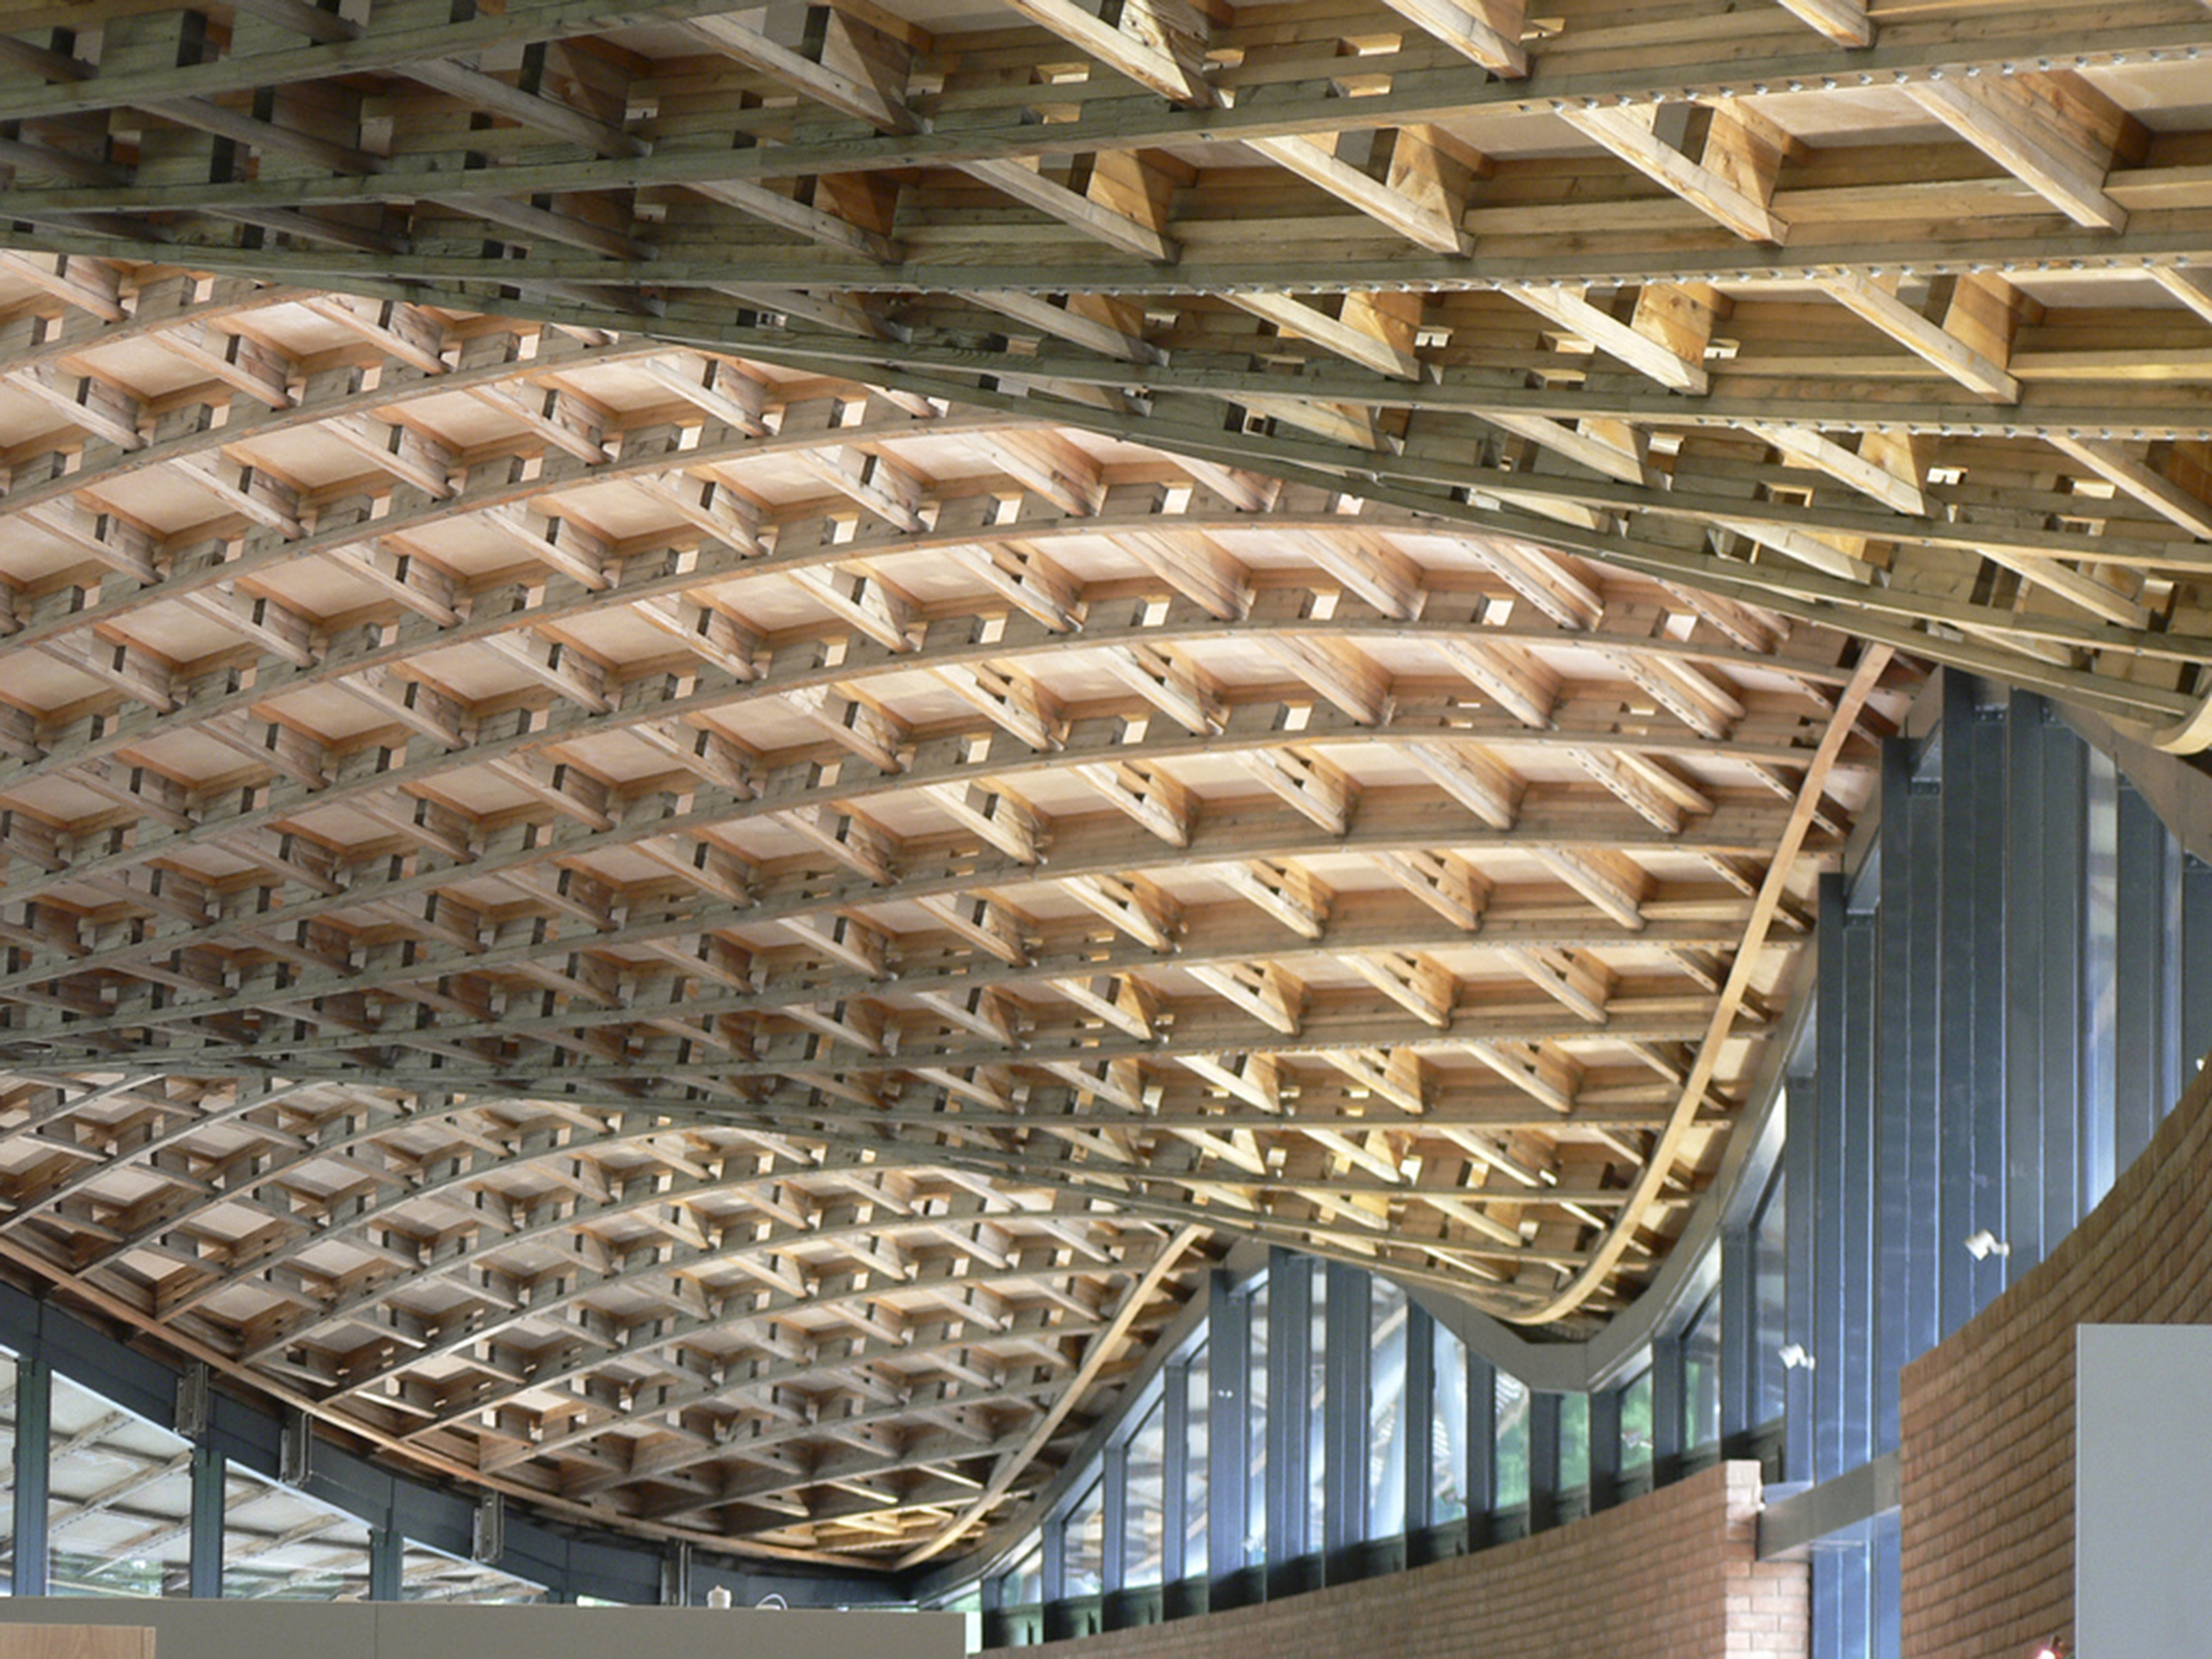
\includegraphics[width=\textwidth]{savill_b.jpg}
		\caption{Interior view}
		\label{fig:savill_a}
	\end{subfigure}%
	\hspace{\MediaGutterWidth}%
	\begin{subfigure}[b]{\TwoMediaWidth}
		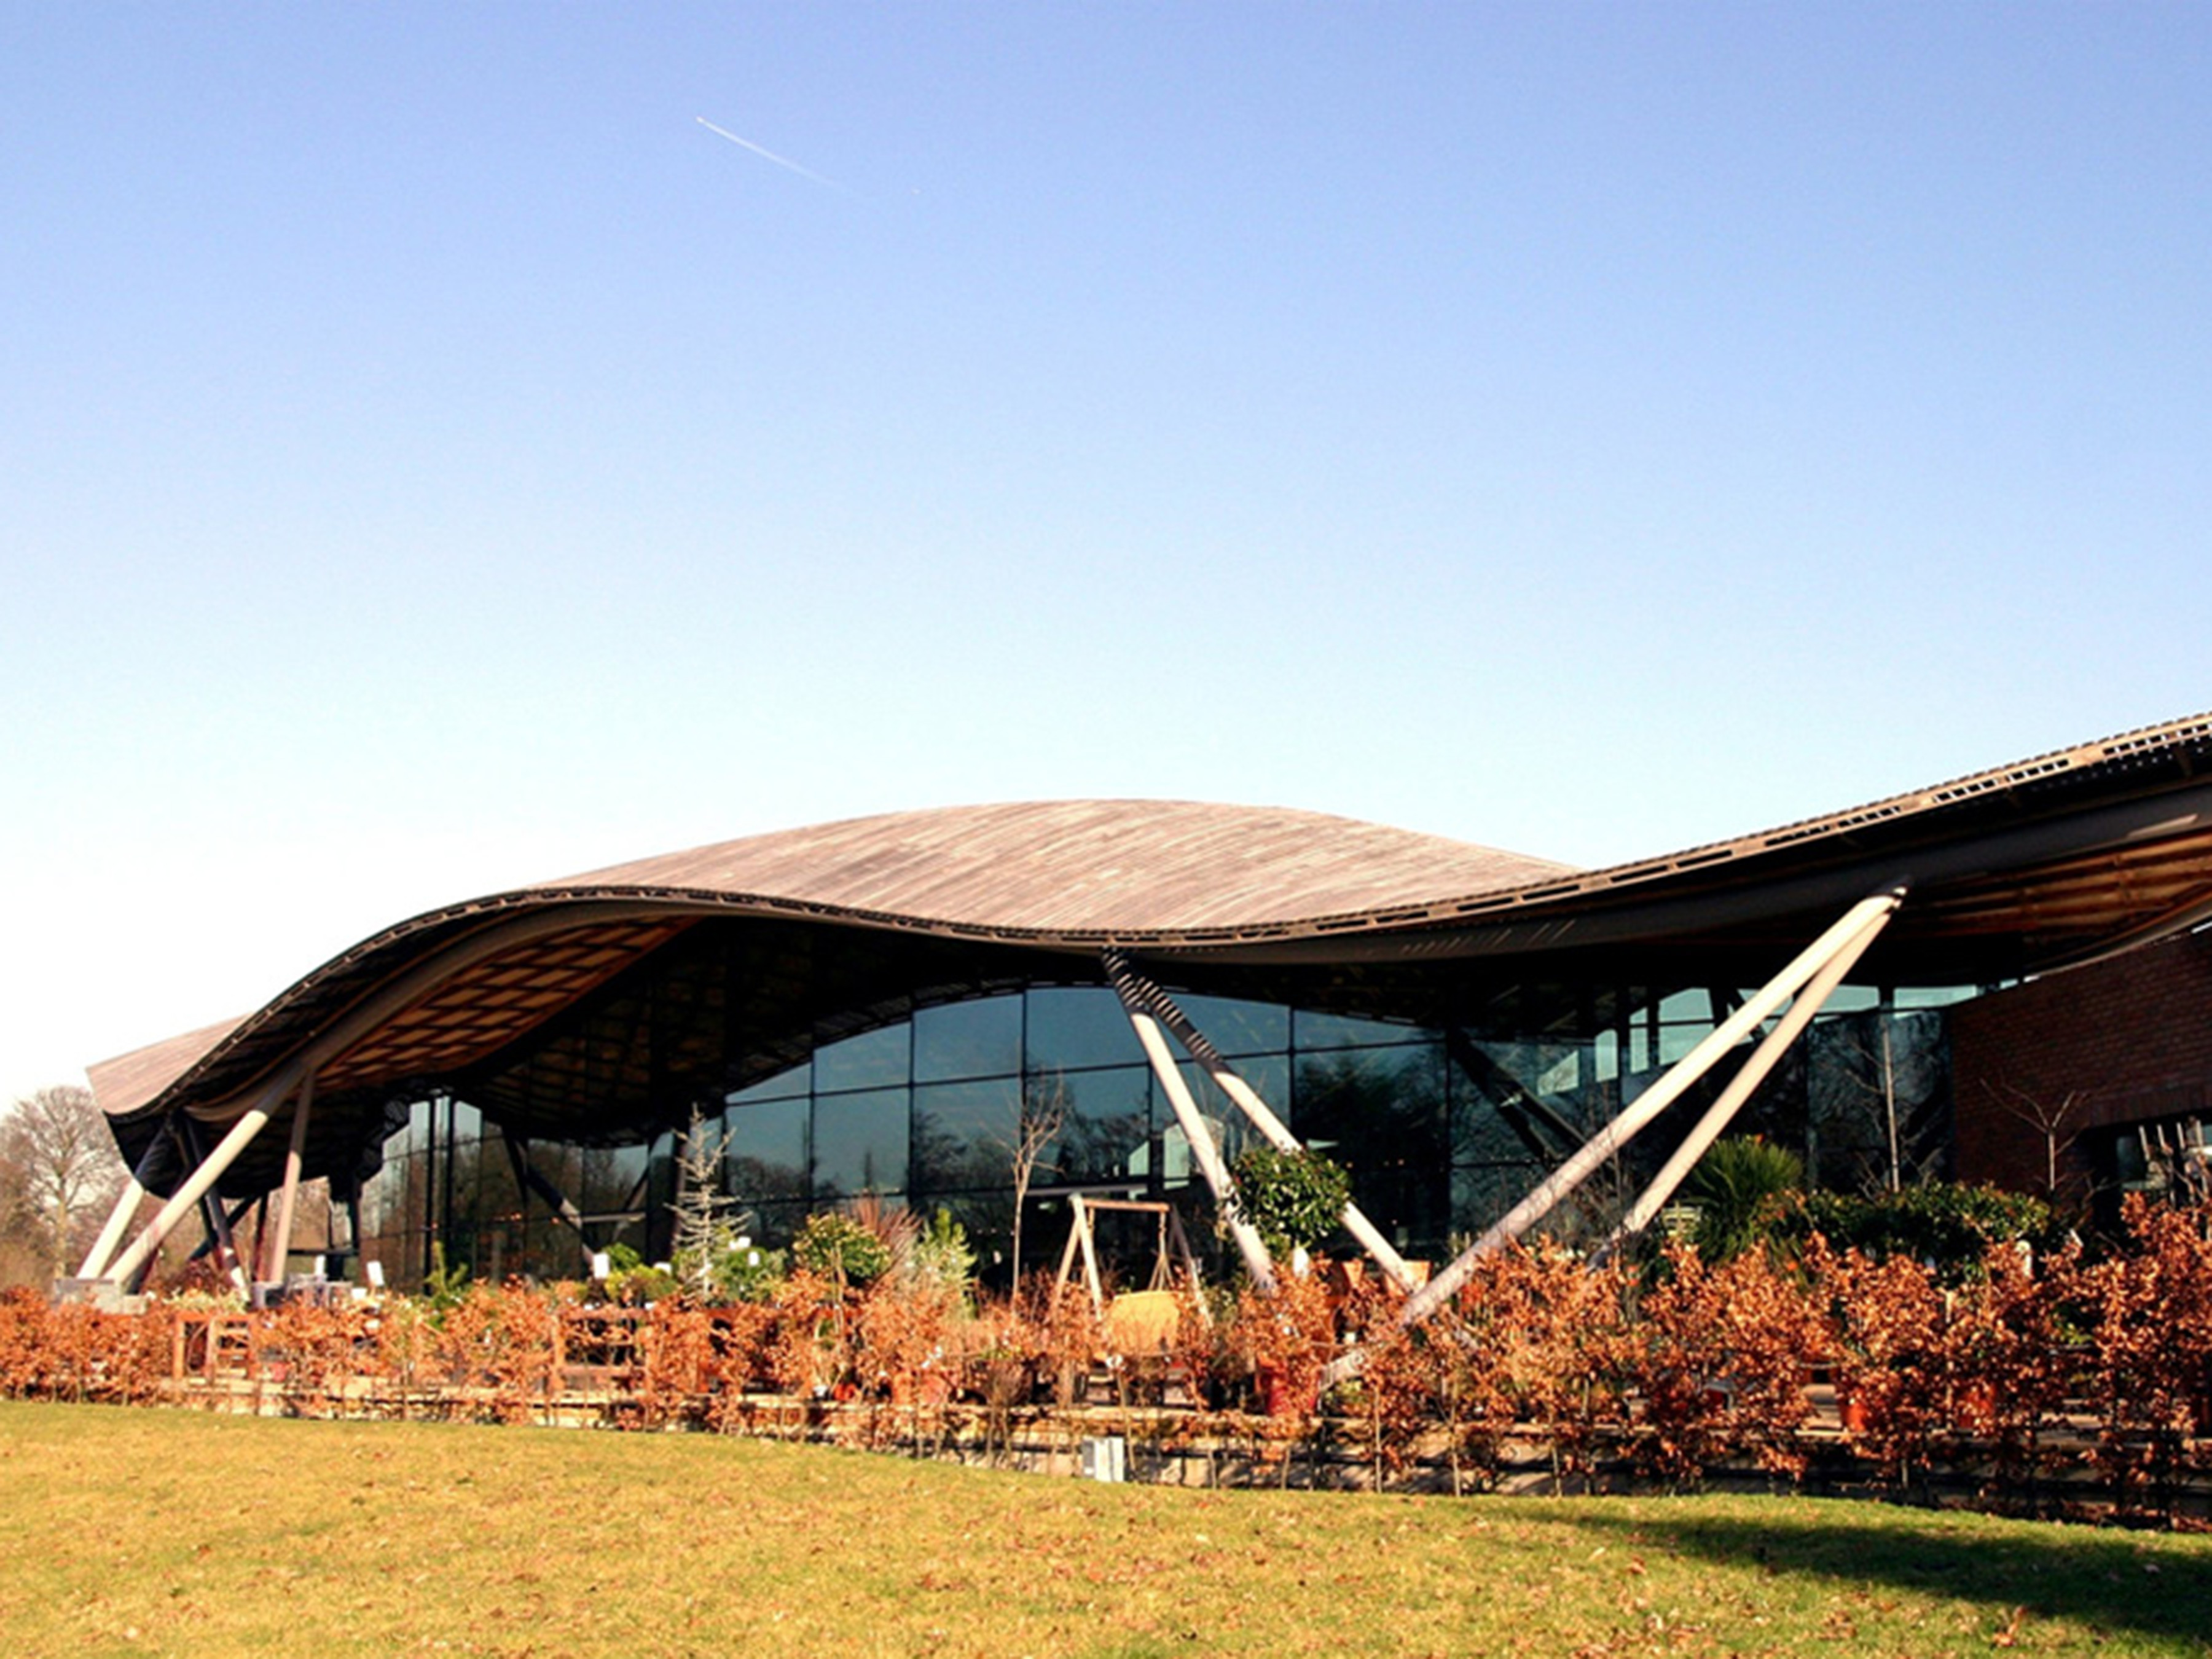
\includegraphics[width=\textwidth]{savill_a.jpg}
		\caption{Exterior view}
		\label{fig:savill_b}
	\end{subfigure}
	\caption[Timber gridshell built in 2006 in Savill, England]{Timber gridshell built in 2006 in Savill, England.}
	\label{fig:savill}
	%
	%
	% \hrule
\end{figure}

\clearpage
\begin{tikzpicture}[remember picture,overlay]
	\node[anchor=north east,inner sep=0pt] at (current page.north east)
	{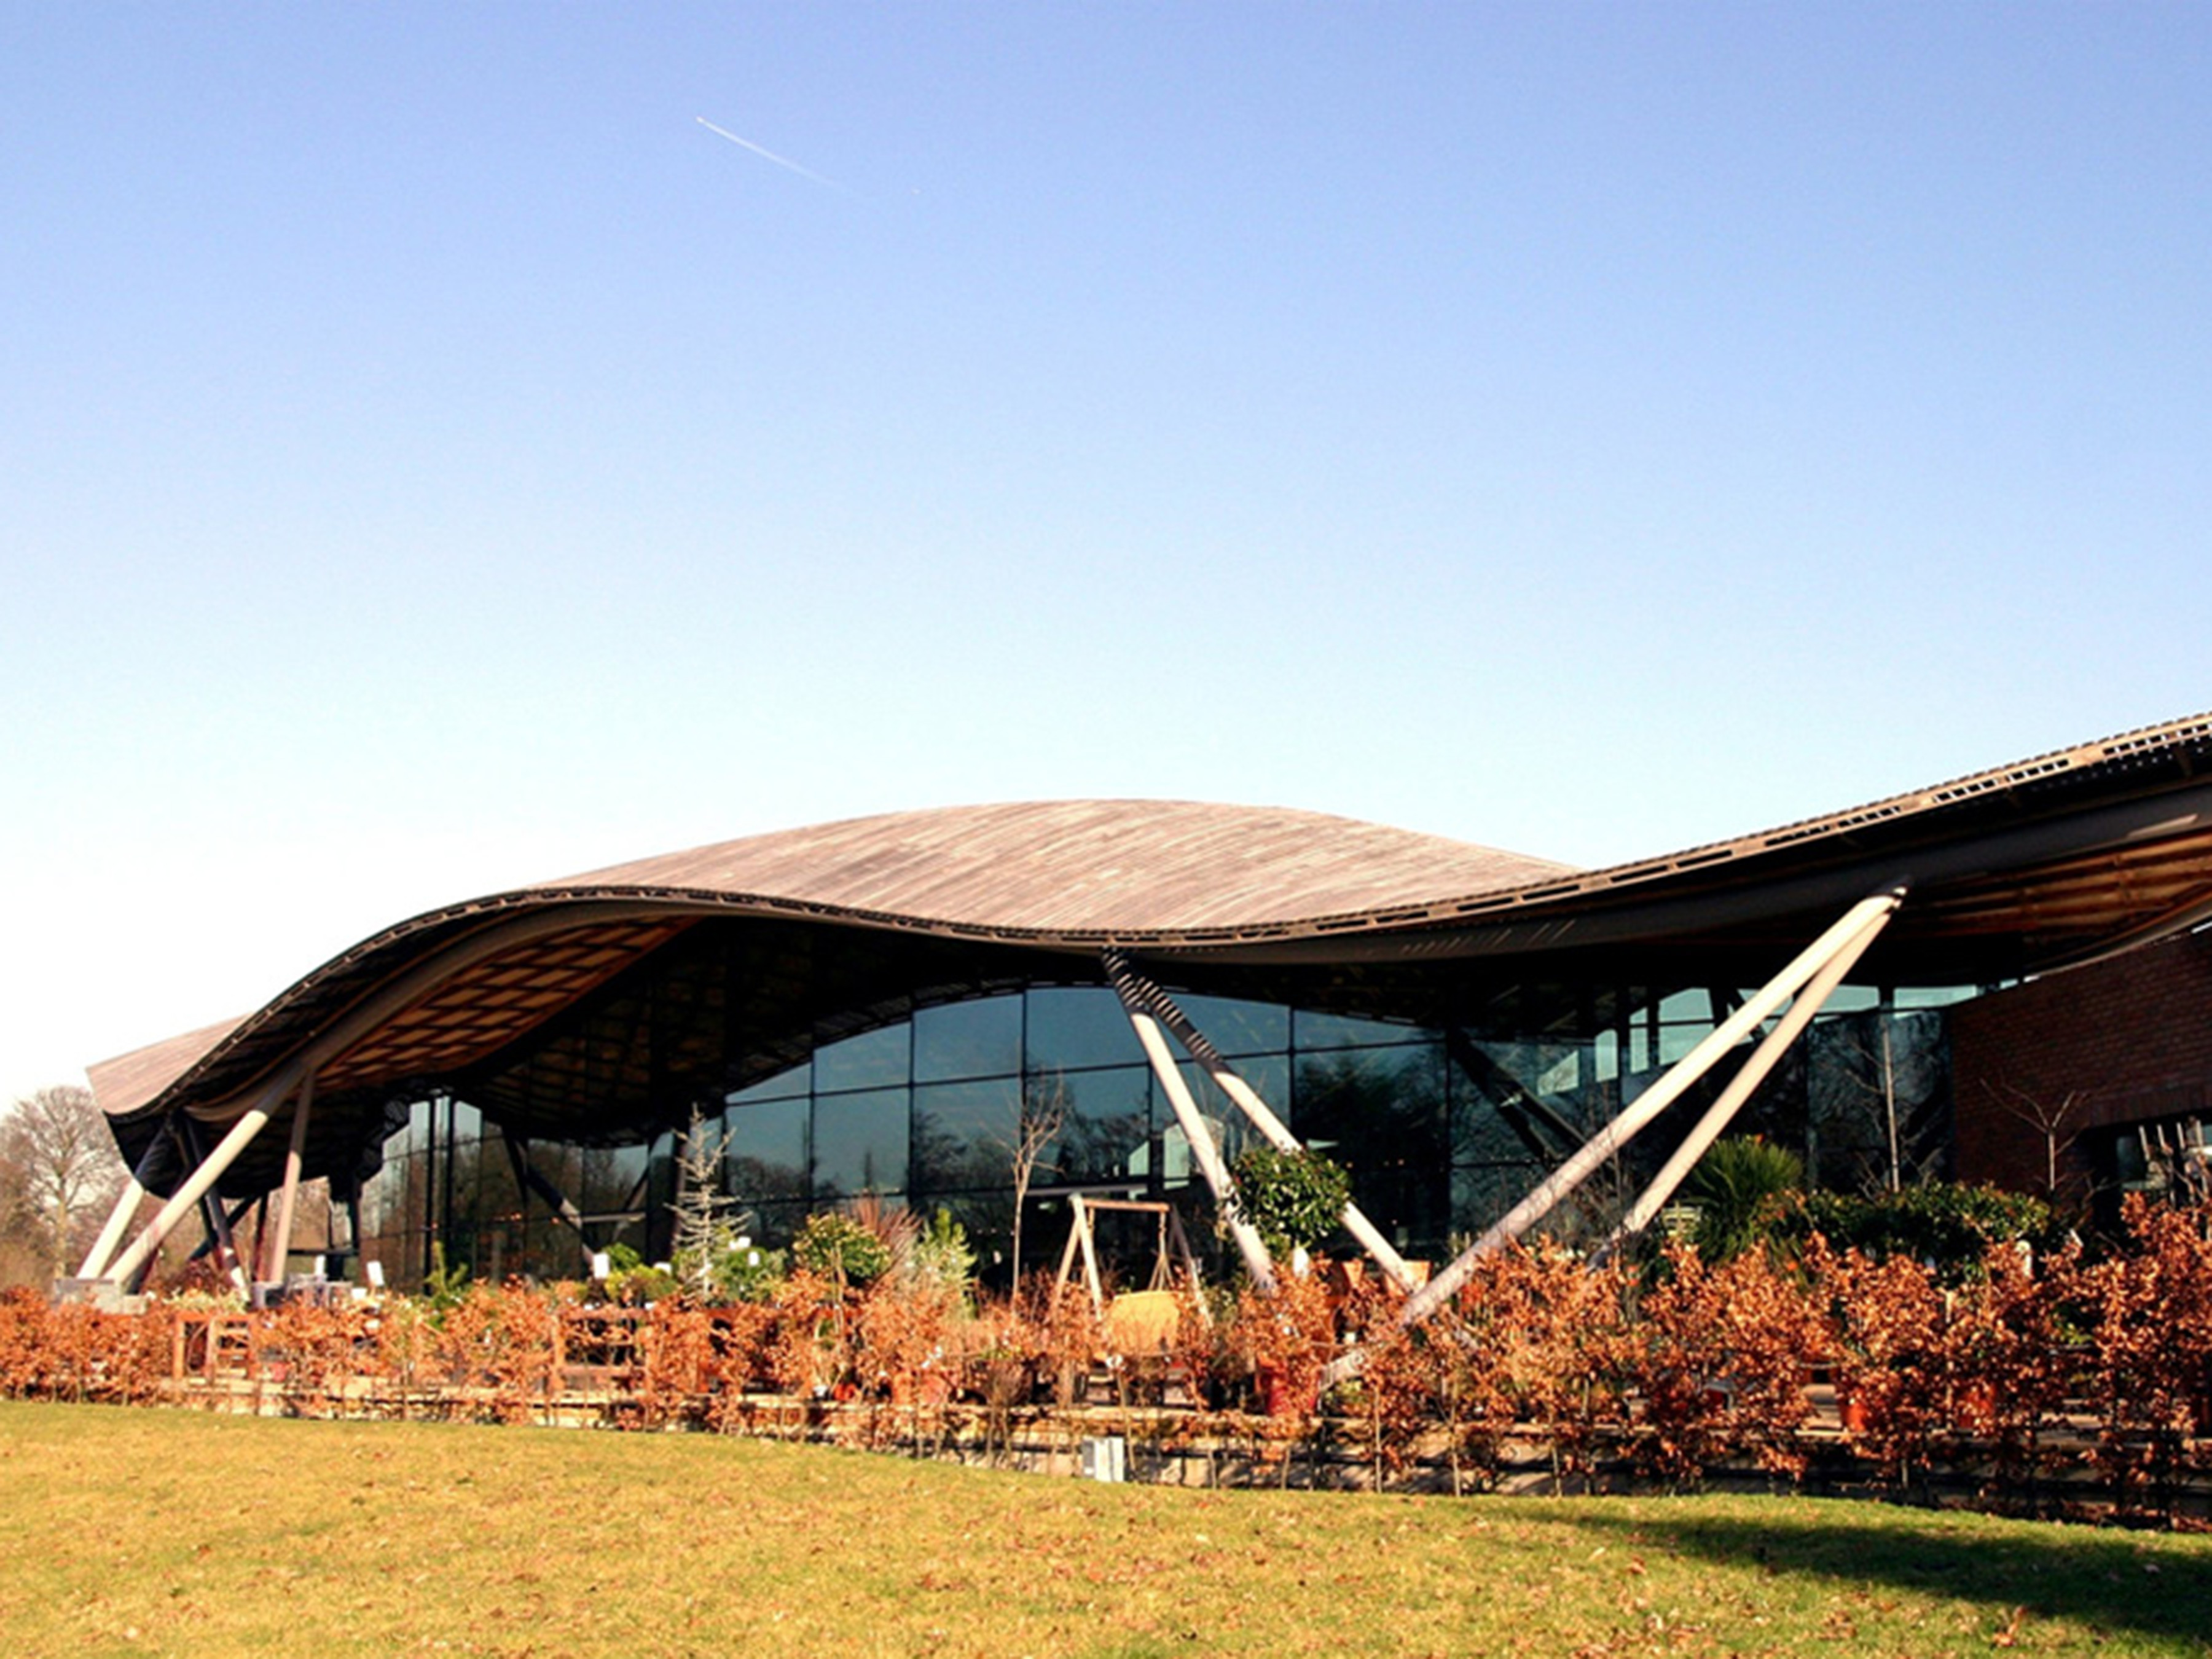
\includegraphics[width=\paperwidth]{savill_a.jpg}};
\end{tikzpicture}

\clearpage
\begin{tikzpicture}[remember picture,overlay]
	\node[anchor=north east,inner sep=0pt] at (current page.north east)
	{
	\begin{minipage}{5cm}
		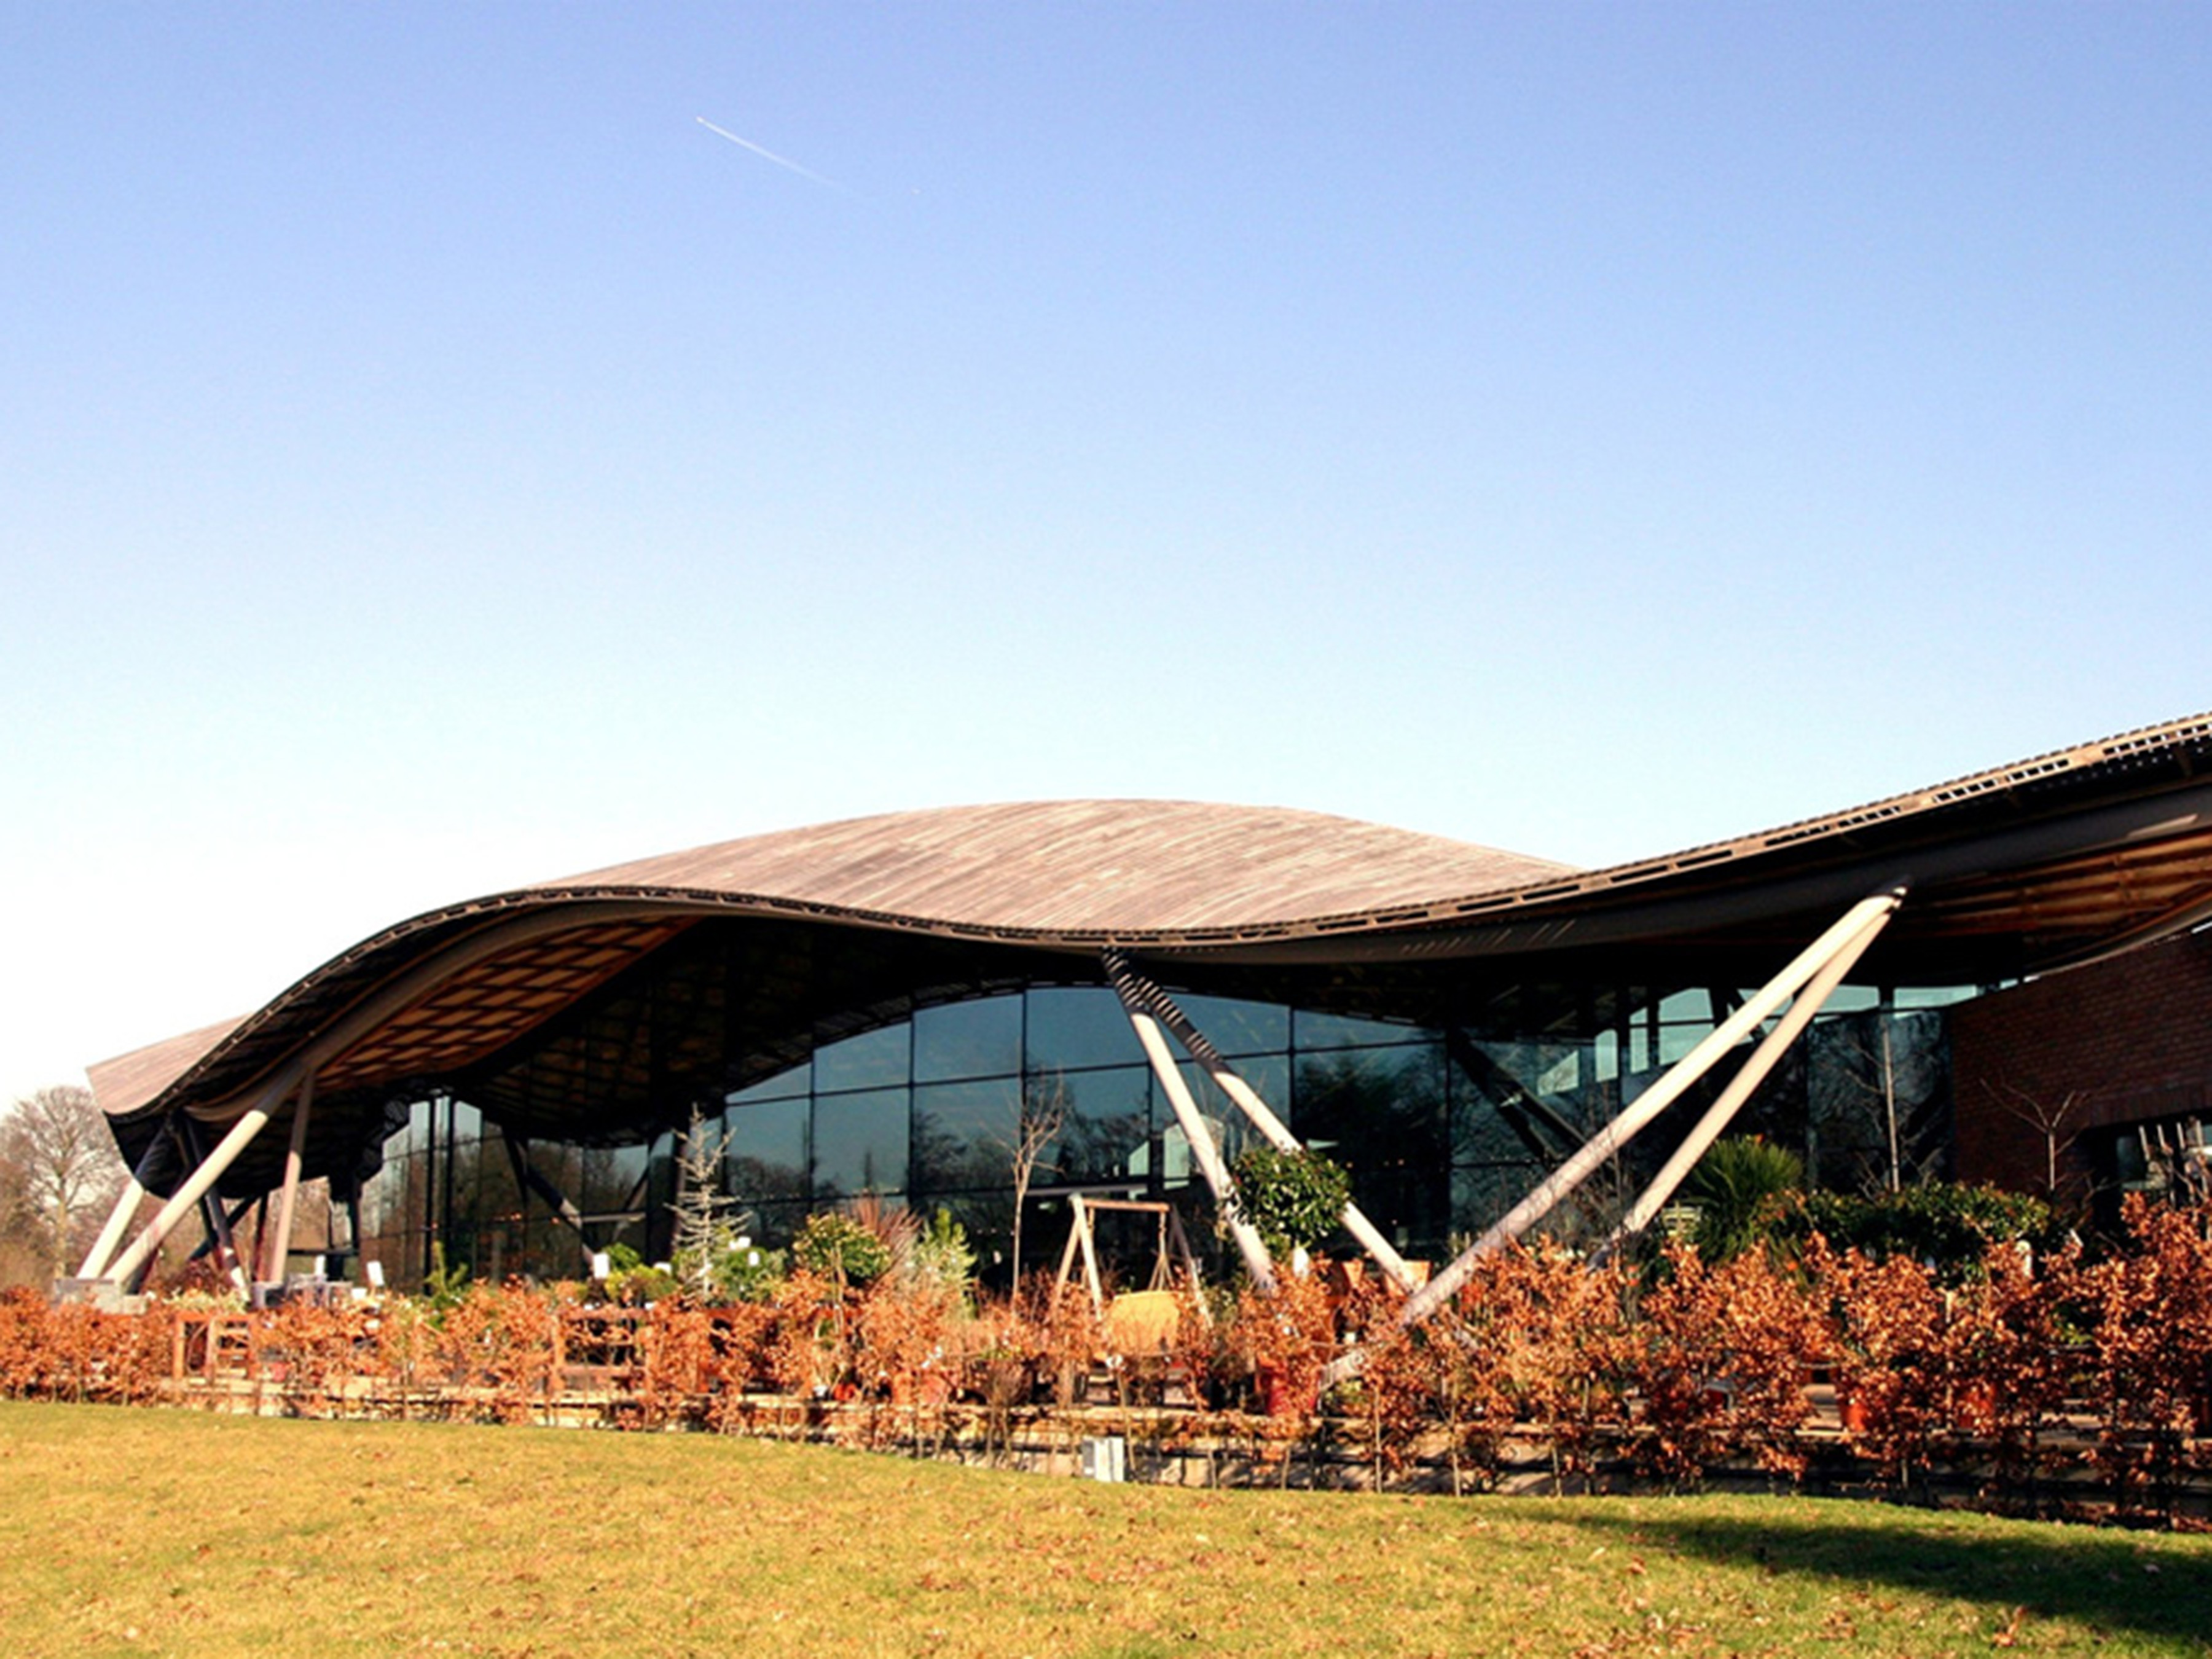
\includegraphics[width=\paperwidth]{savill_a.jpg}
		\captionof{figure}{Some here}
	\end{minipage}
	};
\end{tikzpicture}

\clearpage
\begin{tikzpicture}[remember picture,overlay]
	\node[anchor=north west,inner sep=0pt] at (current page.north west)
	{
	\begin{minipage}{\textwidth}
		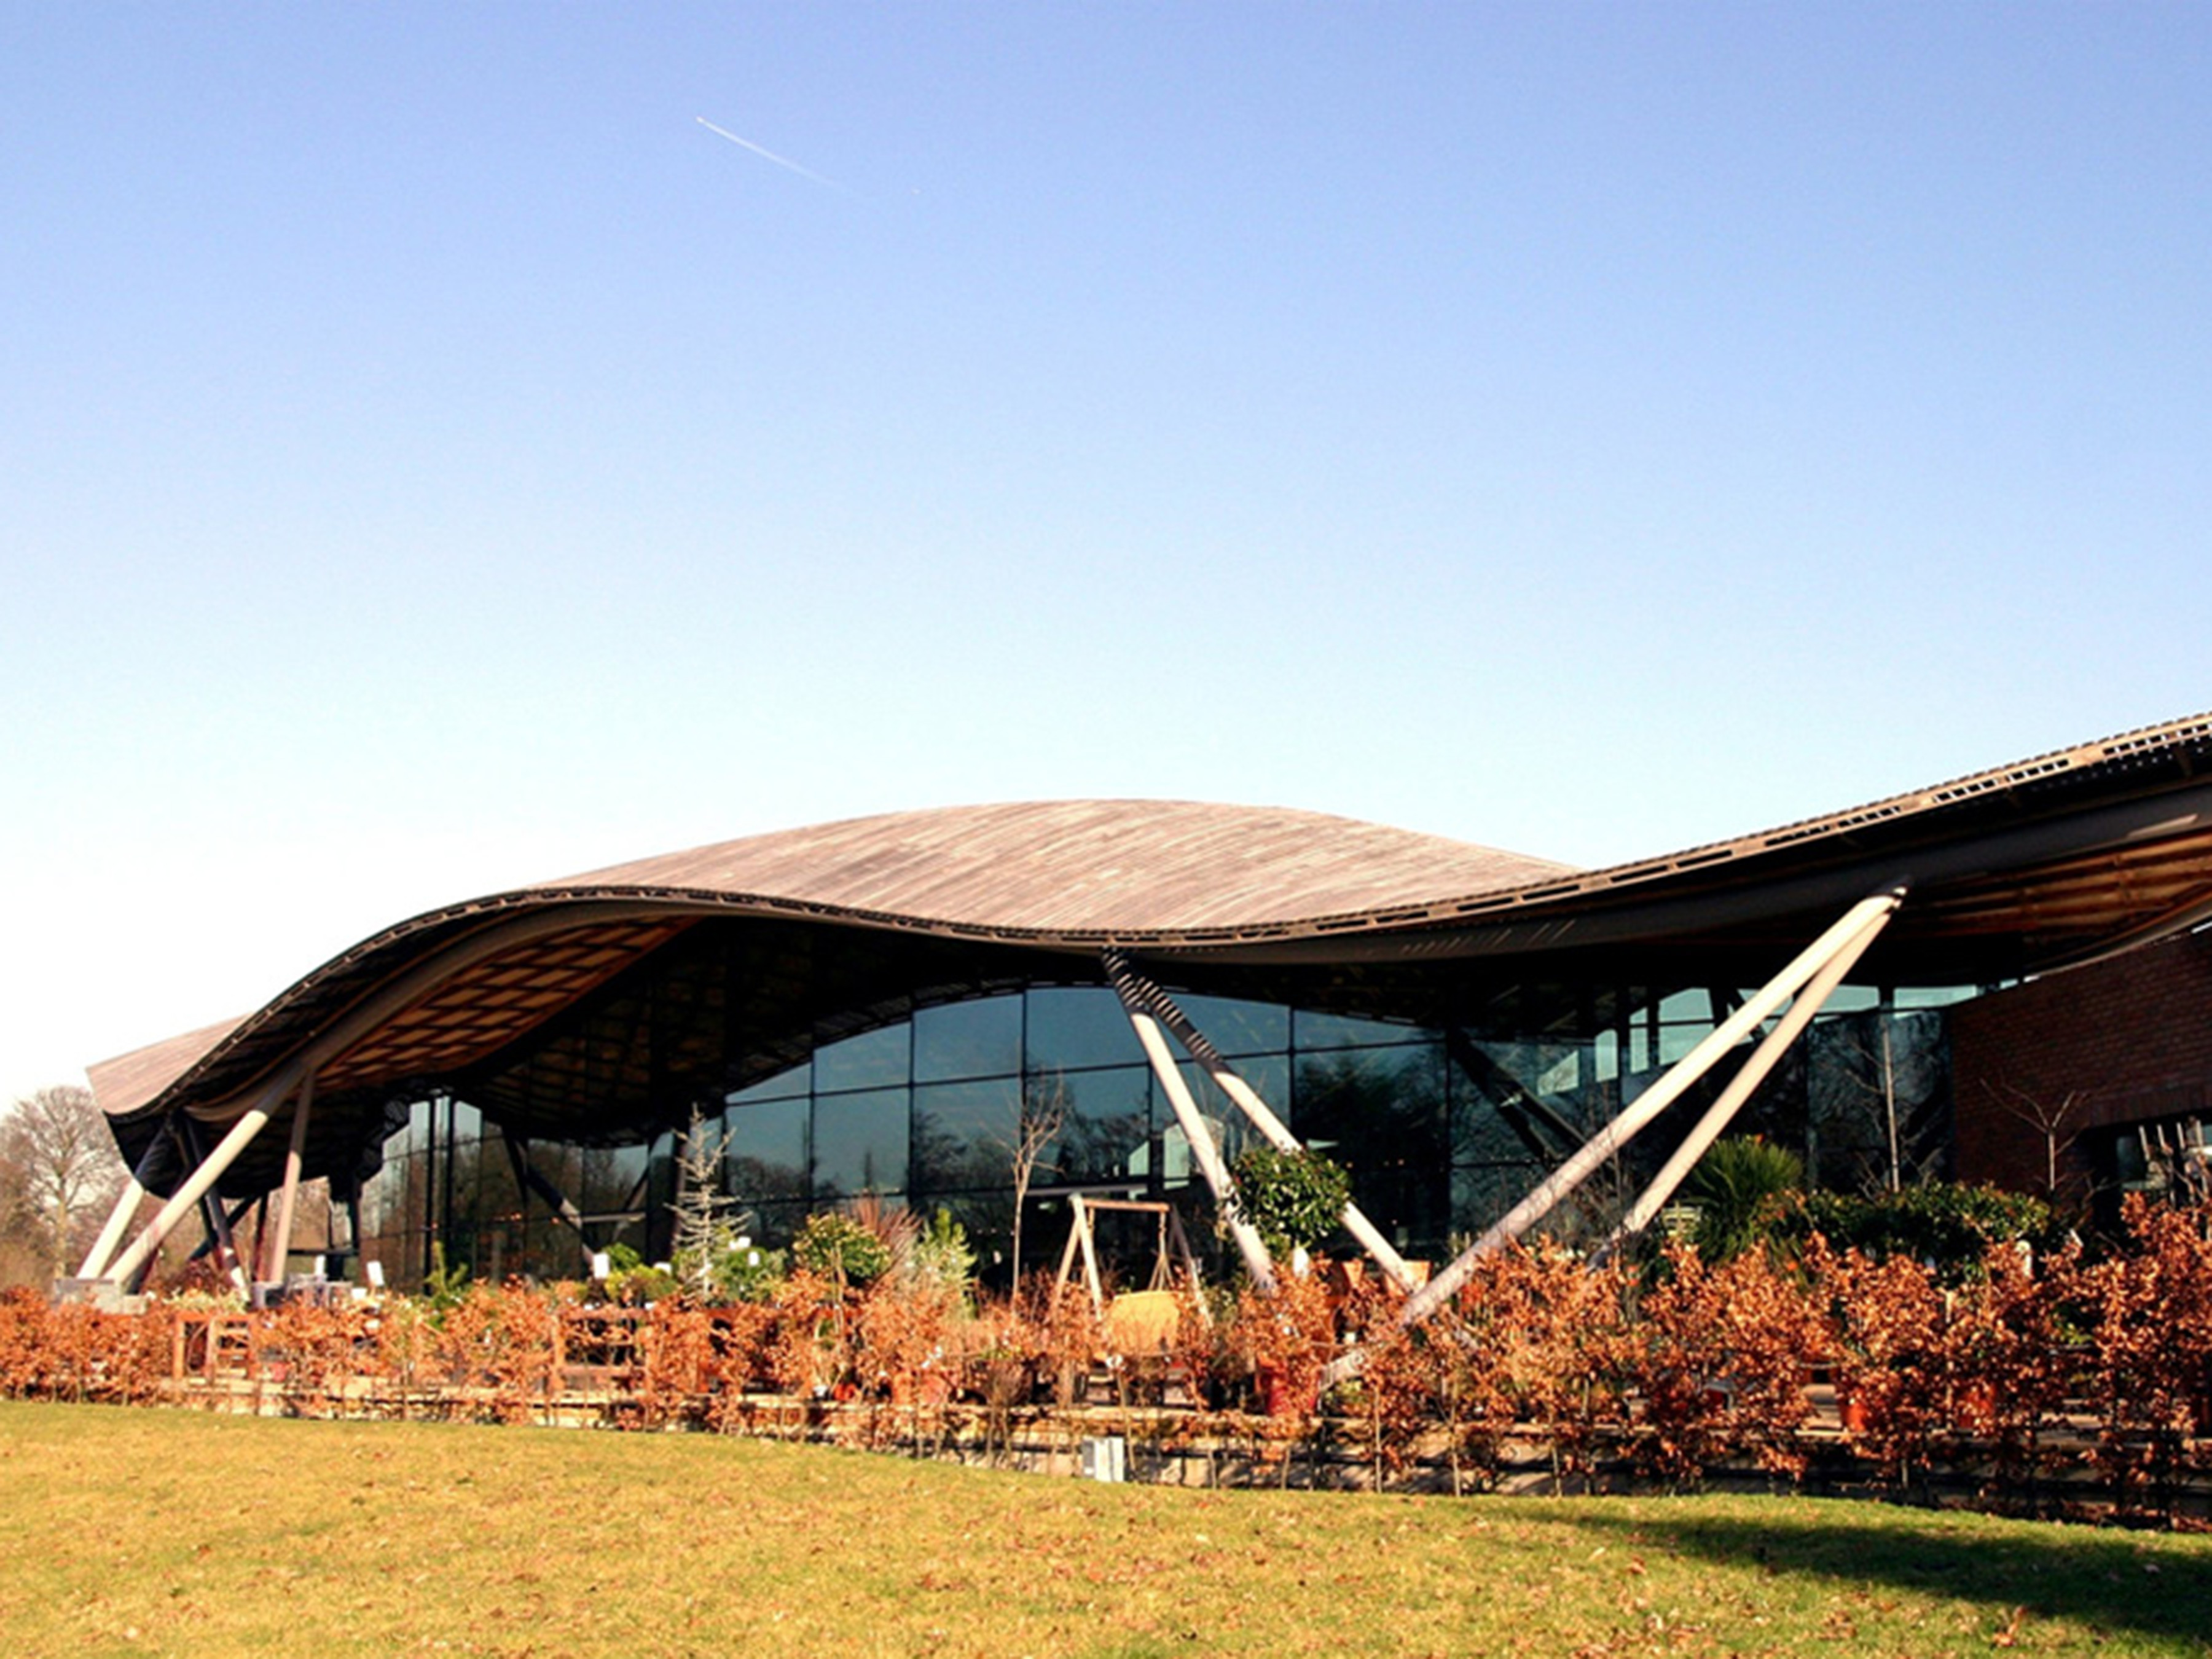
\includegraphics[width=\textwidth]{savill_a.jpg}
		\captionof{subfigure}{}{\label{fig:savill_d}}
	\end{minipage}
	};
\end{tikzpicture}

REF : \cref{fig:savill_d}


% \setlength{\unitlength}{1cm}
% % \begin{picture}(50,50)
% % 	\put(0,0){\hbox{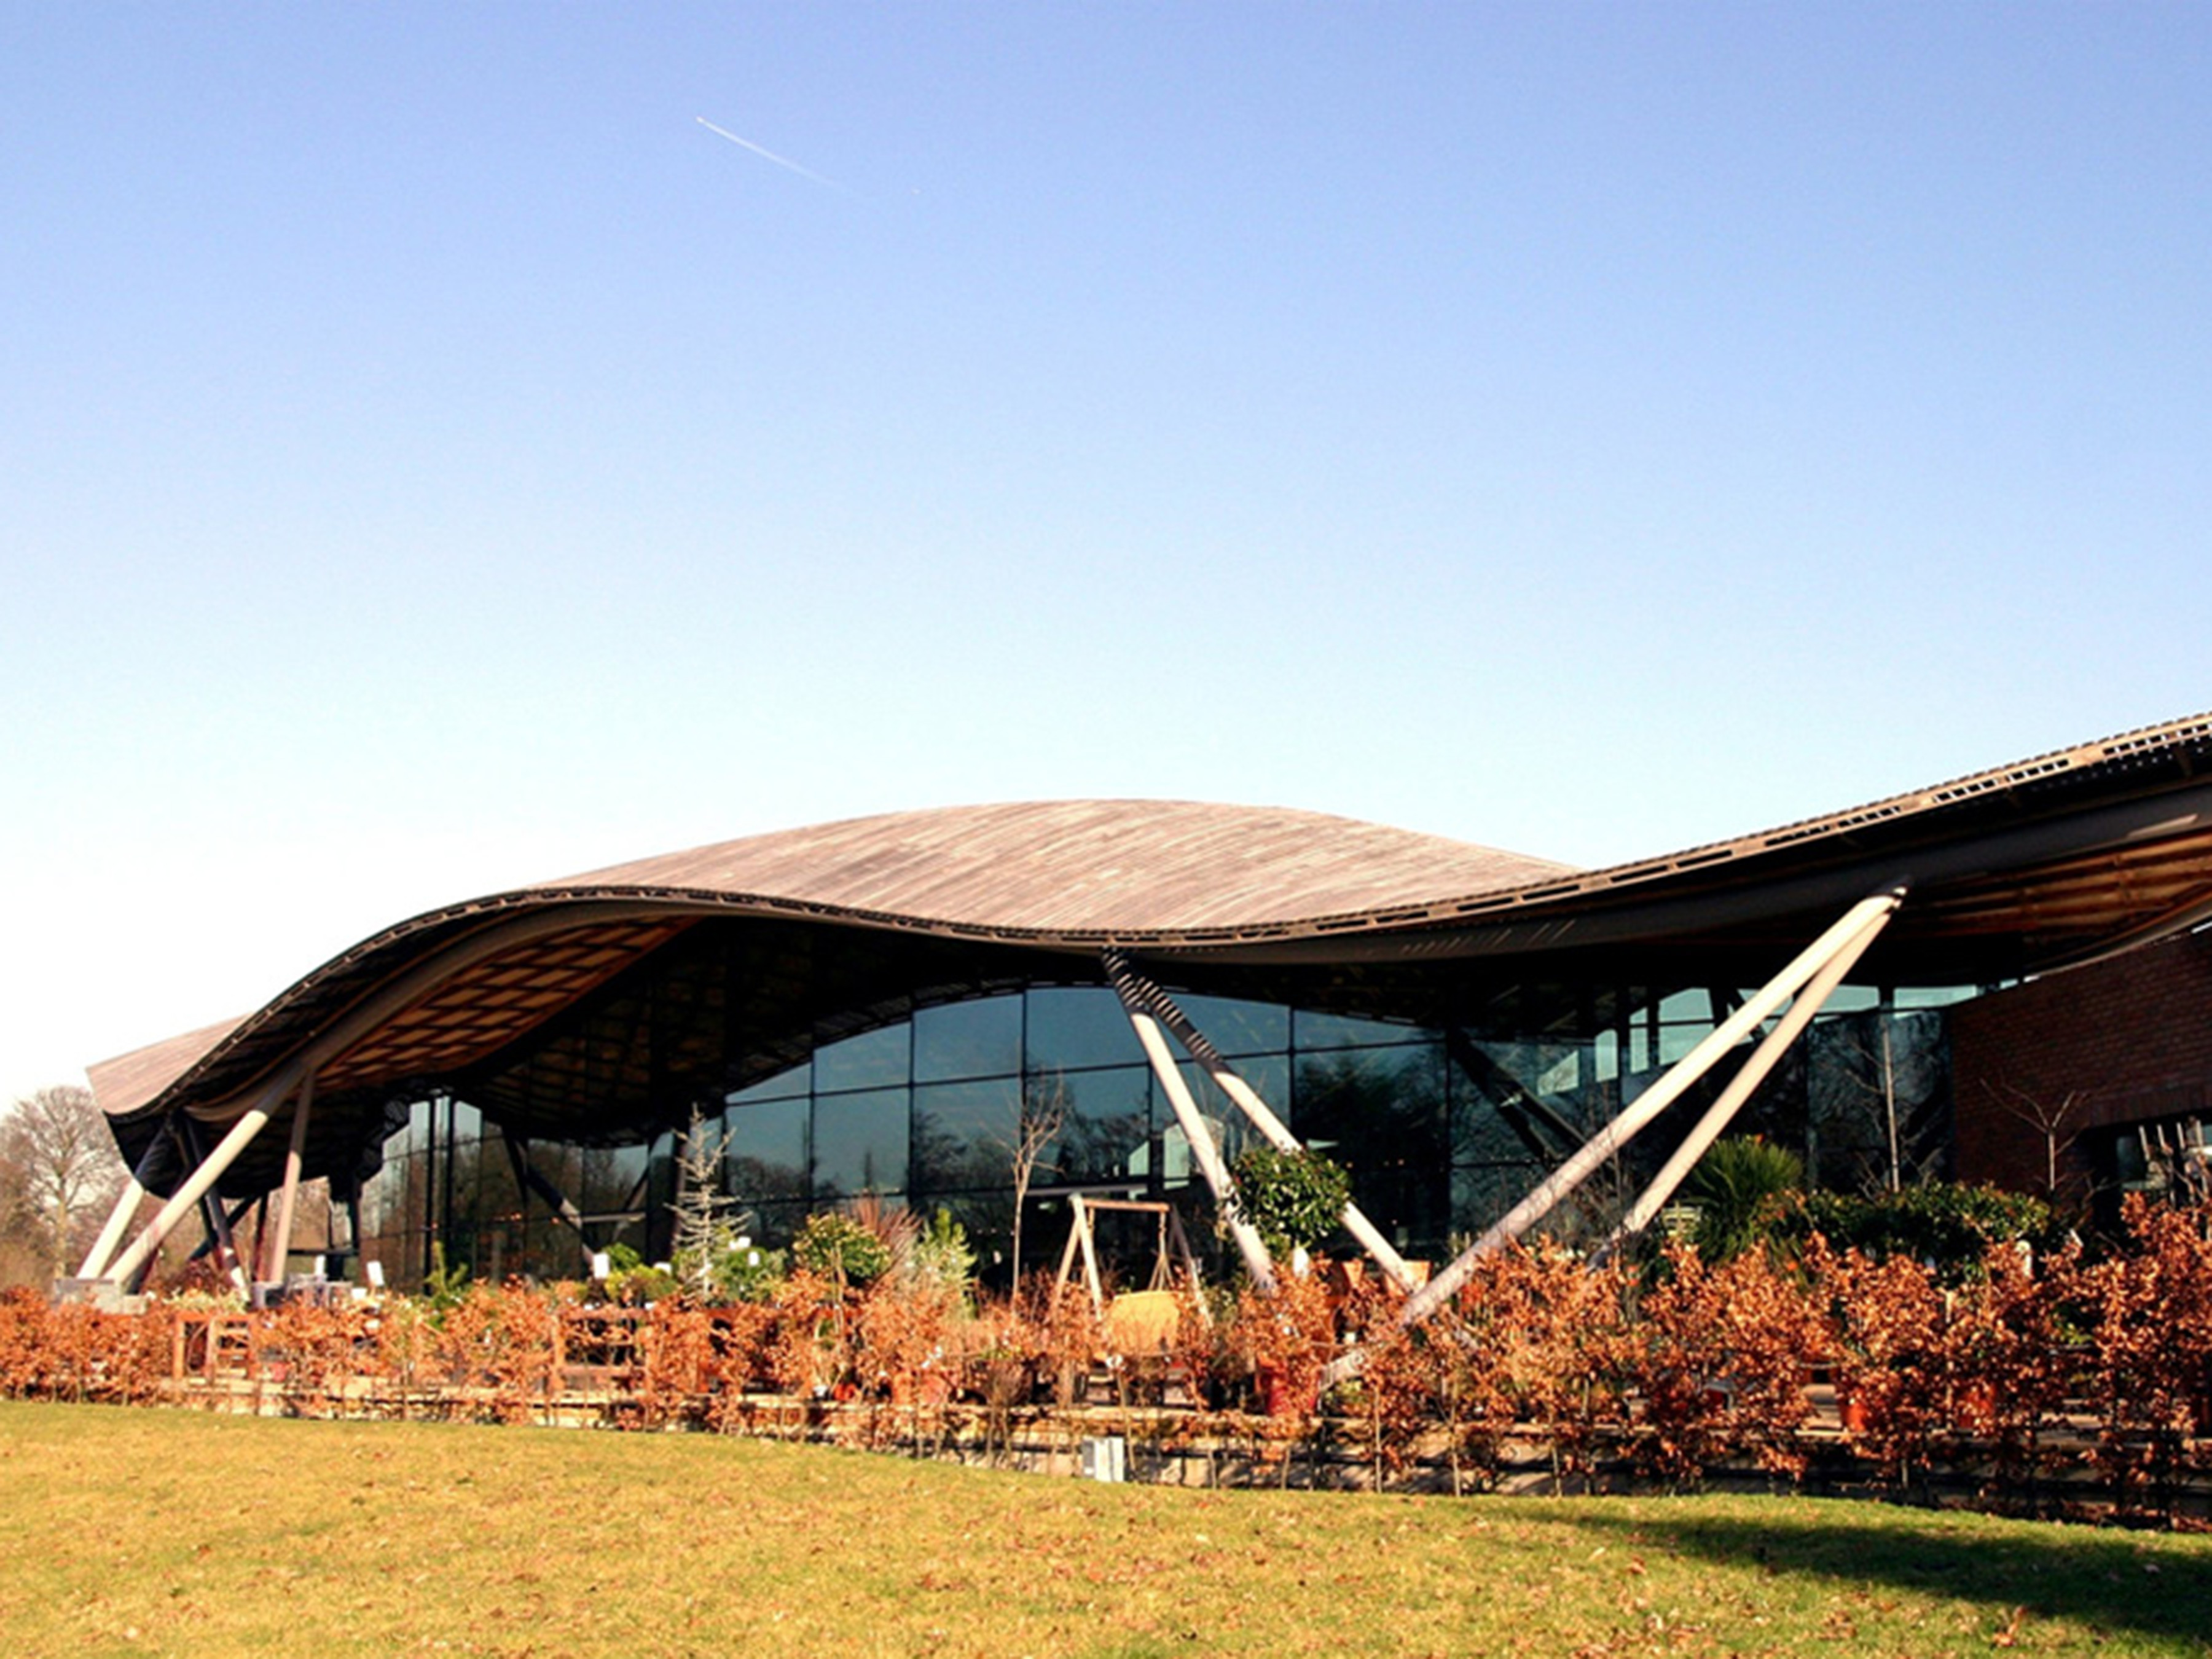
\includegraphics[width=\paperwidth]{savill_a.jpg}}}
% % \end{picture}

% \begin{picture}(0,-10)
% \put(0,0){%
% \begin{minipage}{0.48\linewidth}
% 	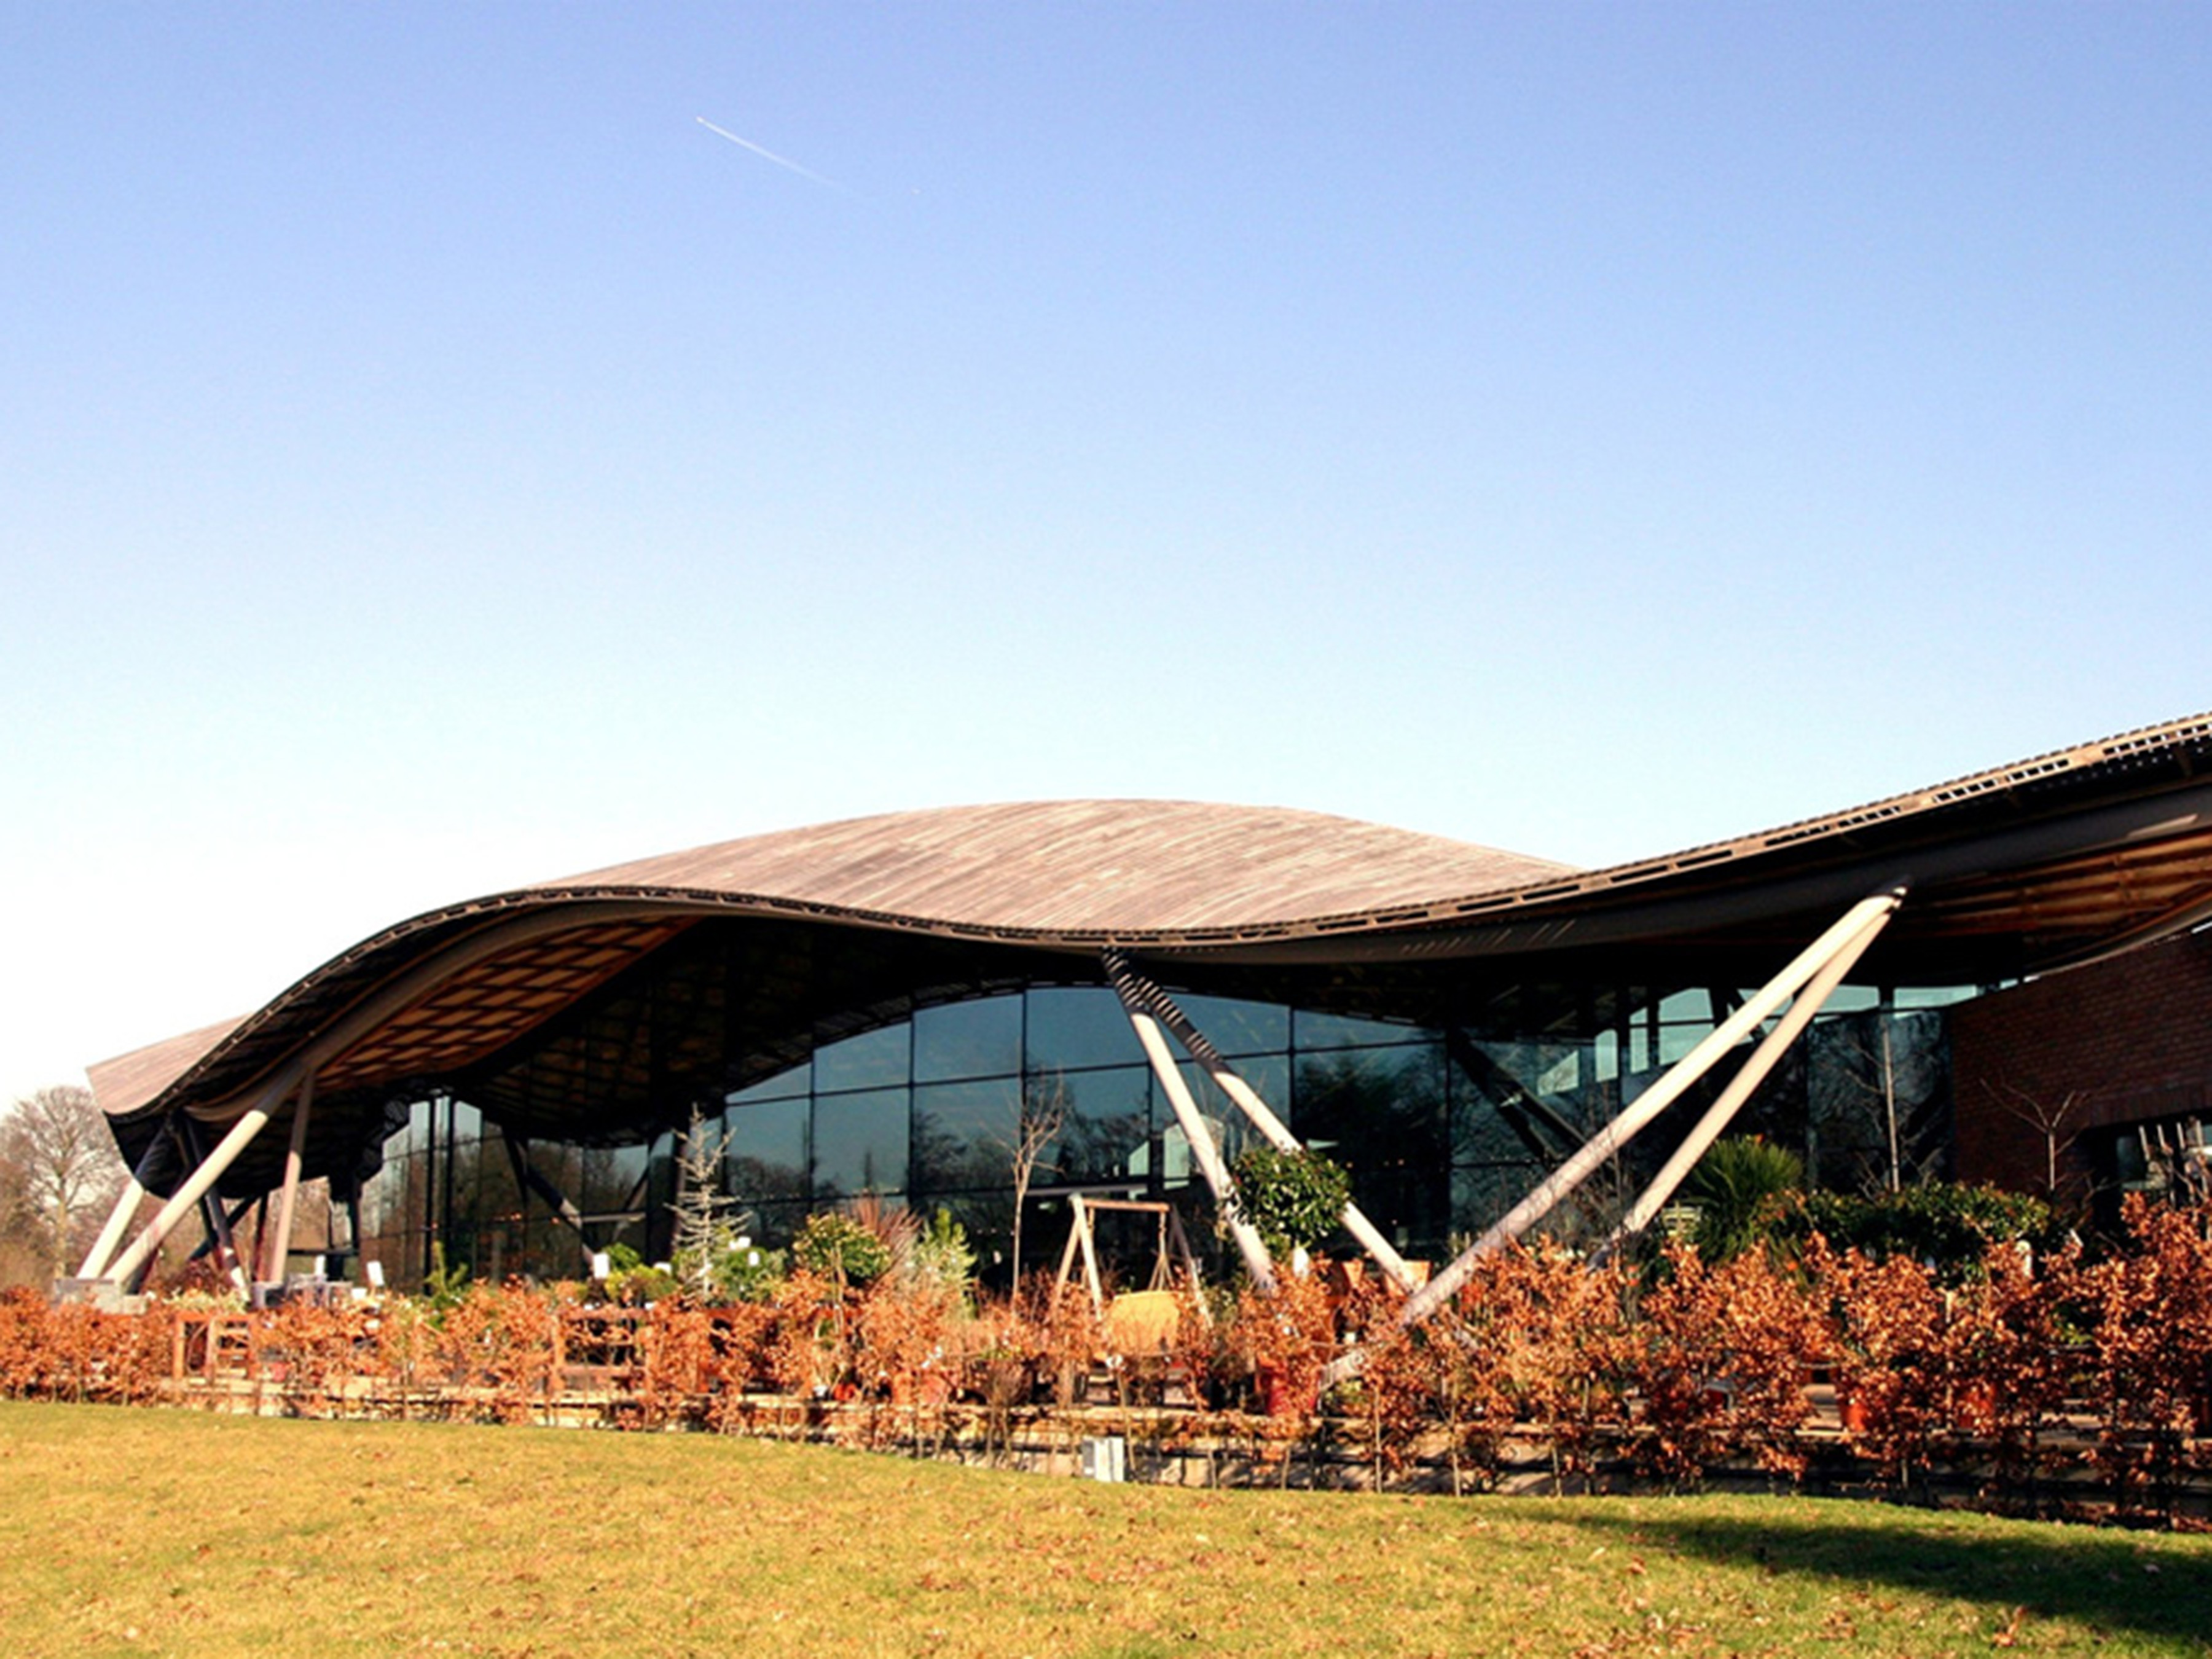
\includegraphics[width=\linewidth]{savill_a.jpg}
% 	\captionof{figure}{Some here}
% \end{minipage}%
% }
% \end{picture}

%  \begin{textblock}{2.5}(\GetX{2cm},\GetY{0cm})
% 	\raggedright
% 	Work is of two kinds: first, altering
% 	the position of matter at or near the
% 	earth’s surface relatively to other such
% 	matter; second, telling other people
% 	to do so.
% \end{textblock}

\begin{textblock*}{10cm}[0,0](0cm,0cm)
	\raggedright
	Work is of two kinds: first, altering
	the position of matter at or near the
	earth’s surface relatively to other such
	matter; second, telling other people
	to do so.
\end{textblock*}

% \begin{textblock}{2.5}[1,1](1,1)
% 	\raggedright
% 	Work is of two kinds: first, altering
% 	the position of matter at or near the
% 	earth’s surface relatively to other such
% 	matter; second, telling other people
% 	to do so.
% \end{textblock}



%
%\begin{figure}[p]
%     	\centering
%%	\begin{fullpage}
%		\subfloat[][Interior view]{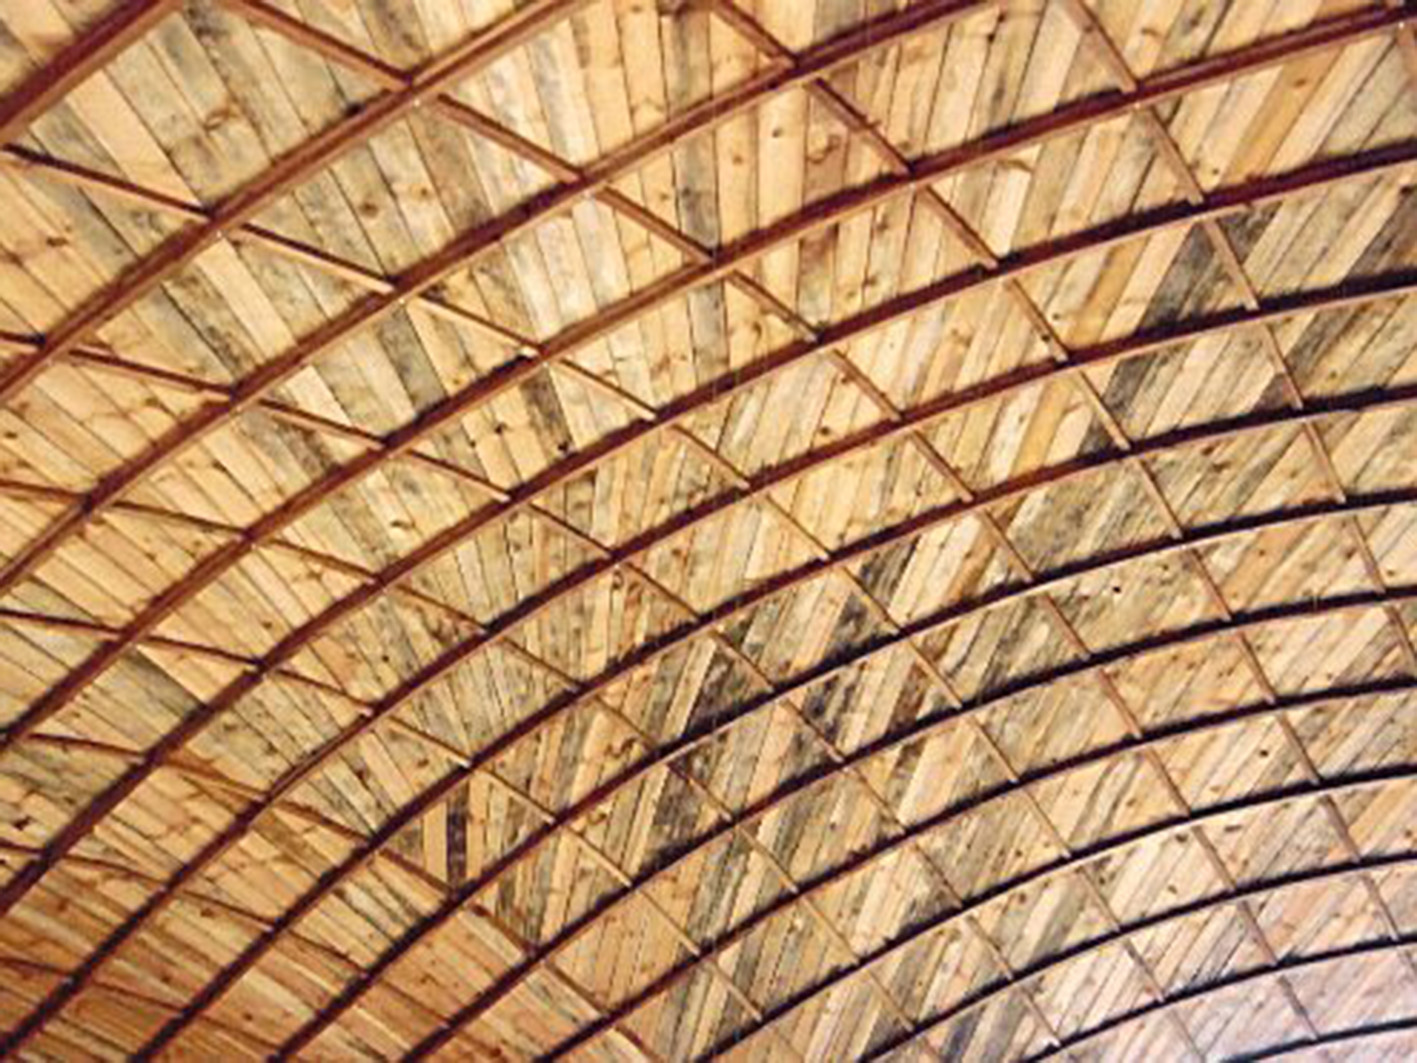
\includegraphics[width=\TwoMediaWidth]{pishwanton_int.jpg}\label{fig:pishwanton_a}}
%		\hspace{\MediaGutterWidth}% (%) required to prevent extra space
%		\subfloat[][Exterior view]{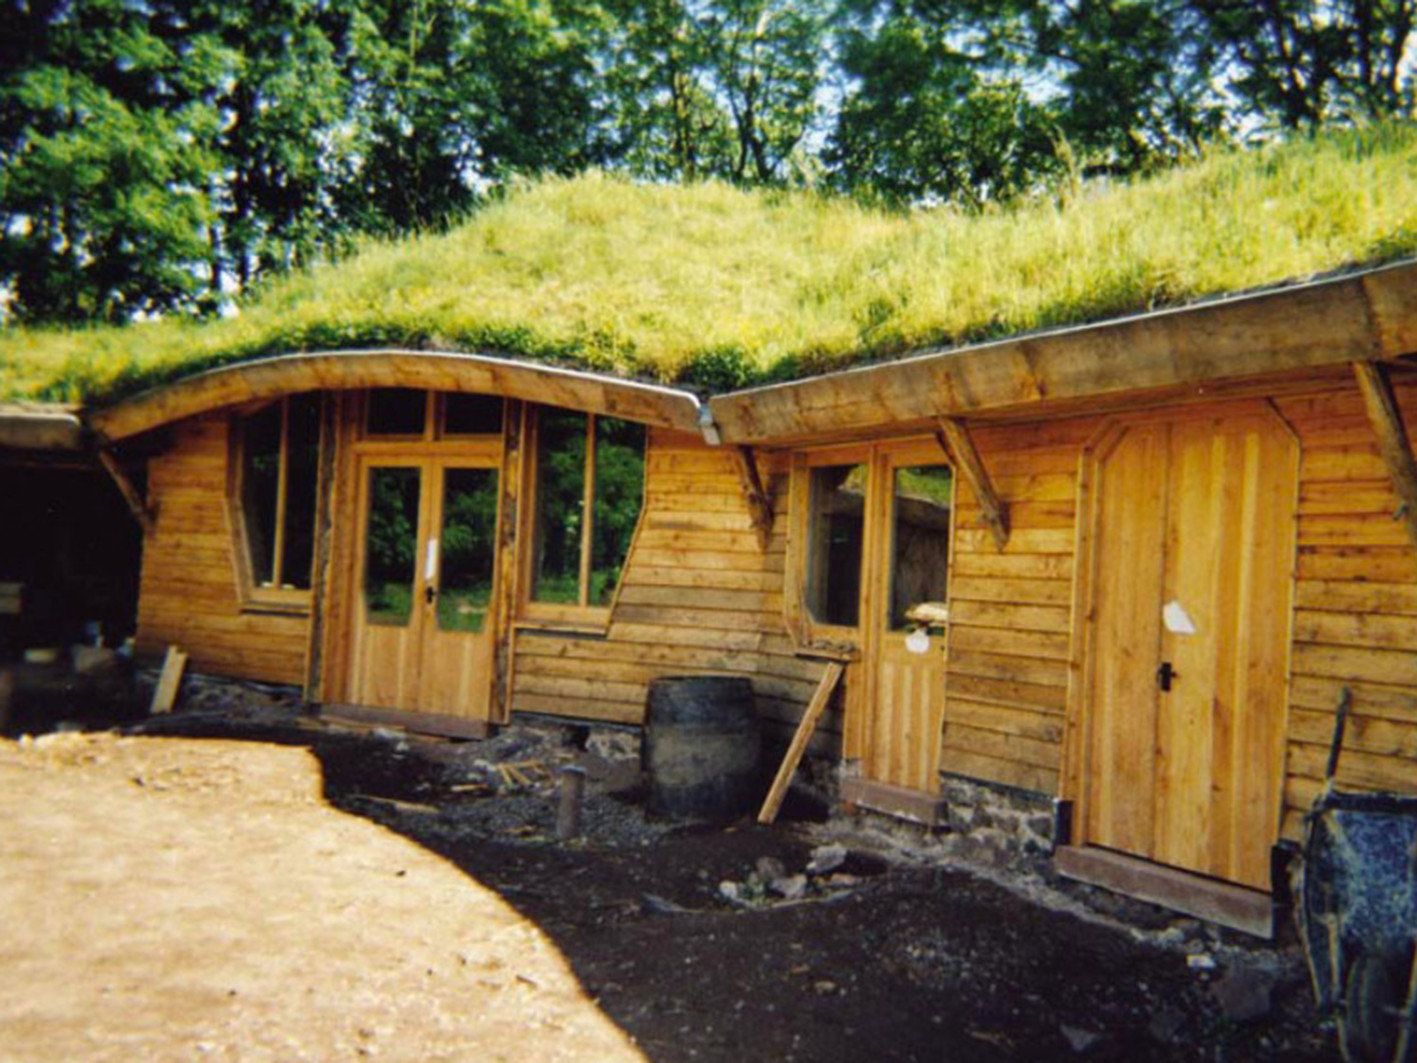
\includegraphics[width=\TwoMediaWidth]{pishwanton_ext.jpg}\label{fig:pishwanton_b}}
%%		\vspace{10pt}
%		\captionof{figure}[Timber gridshell built in 2002 in Pishwanton, England]{Timber gridshell built in 2002 in Pishwanton, England.}
%		\label{fig:pishwanton}
%		%
%		\vspace{\fill}
%		%
%		\subfloat[][Interior view]{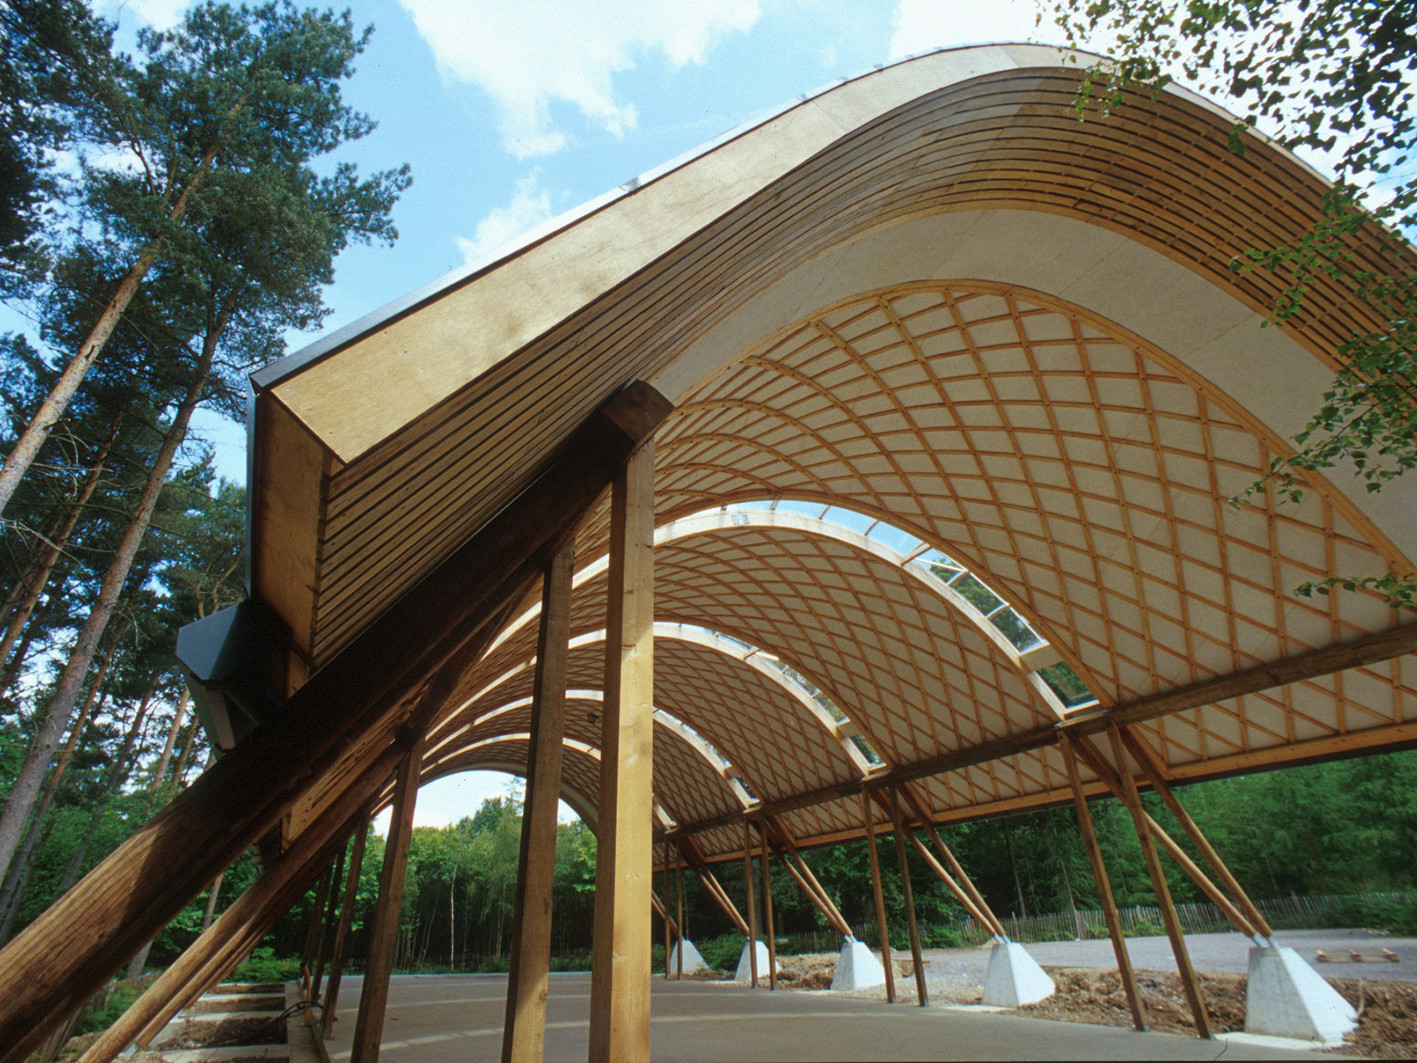
\includegraphics[width=\TwoMediaWidth]{flimwell_int.jpg}\label{fig:flimwell_a}}
%		\hspace{\MediaGutterWidth}% (%) required to prevent extra space
%		\subfloat[][Exterior view]{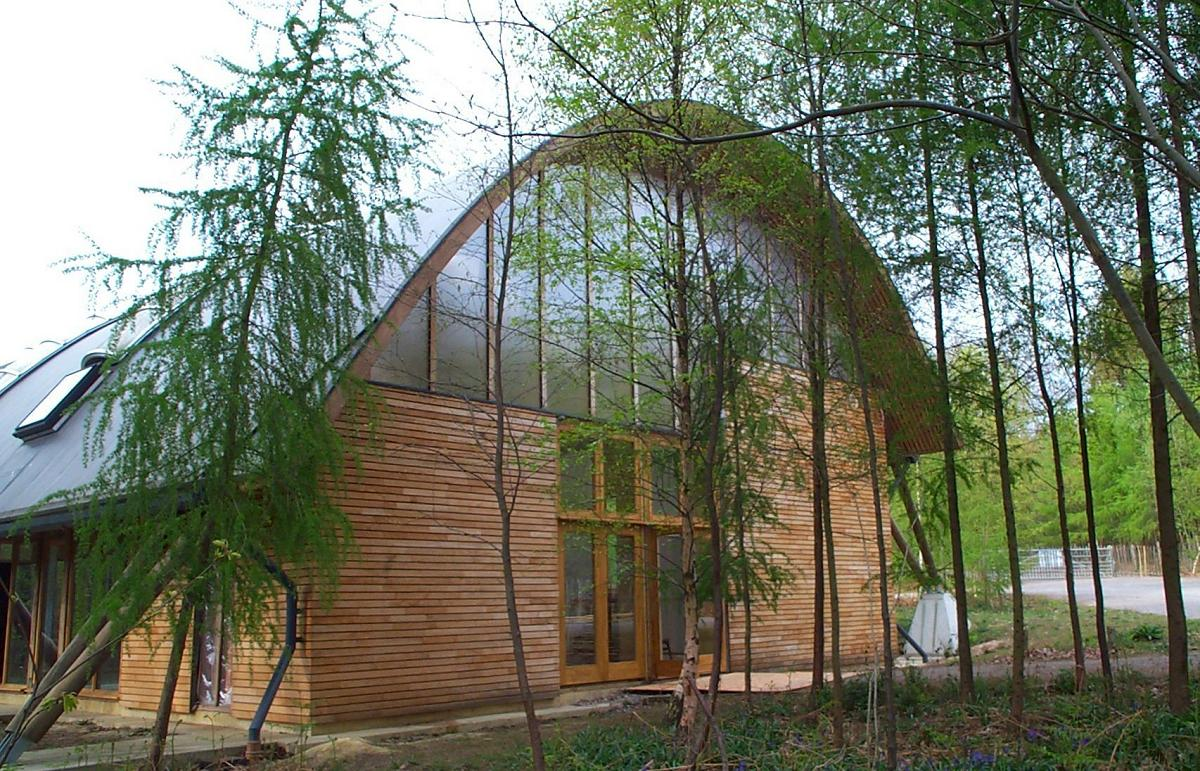
\includegraphics[width=\TwoMediaWidth]{flimwell_ext.jpg}\label{fig:flimwell_b}}
%%		\vspace{10pt}
%		\captionof{figure}[Timber gridshell built in 2003 in Filmwell, England]{Timber gridshell built in 2003 in Filmwell, England.}
%		\label{fig:flimwell}
%		%
%		\vspace{\fill}
%		%
%		\subfloat[][Interior view]{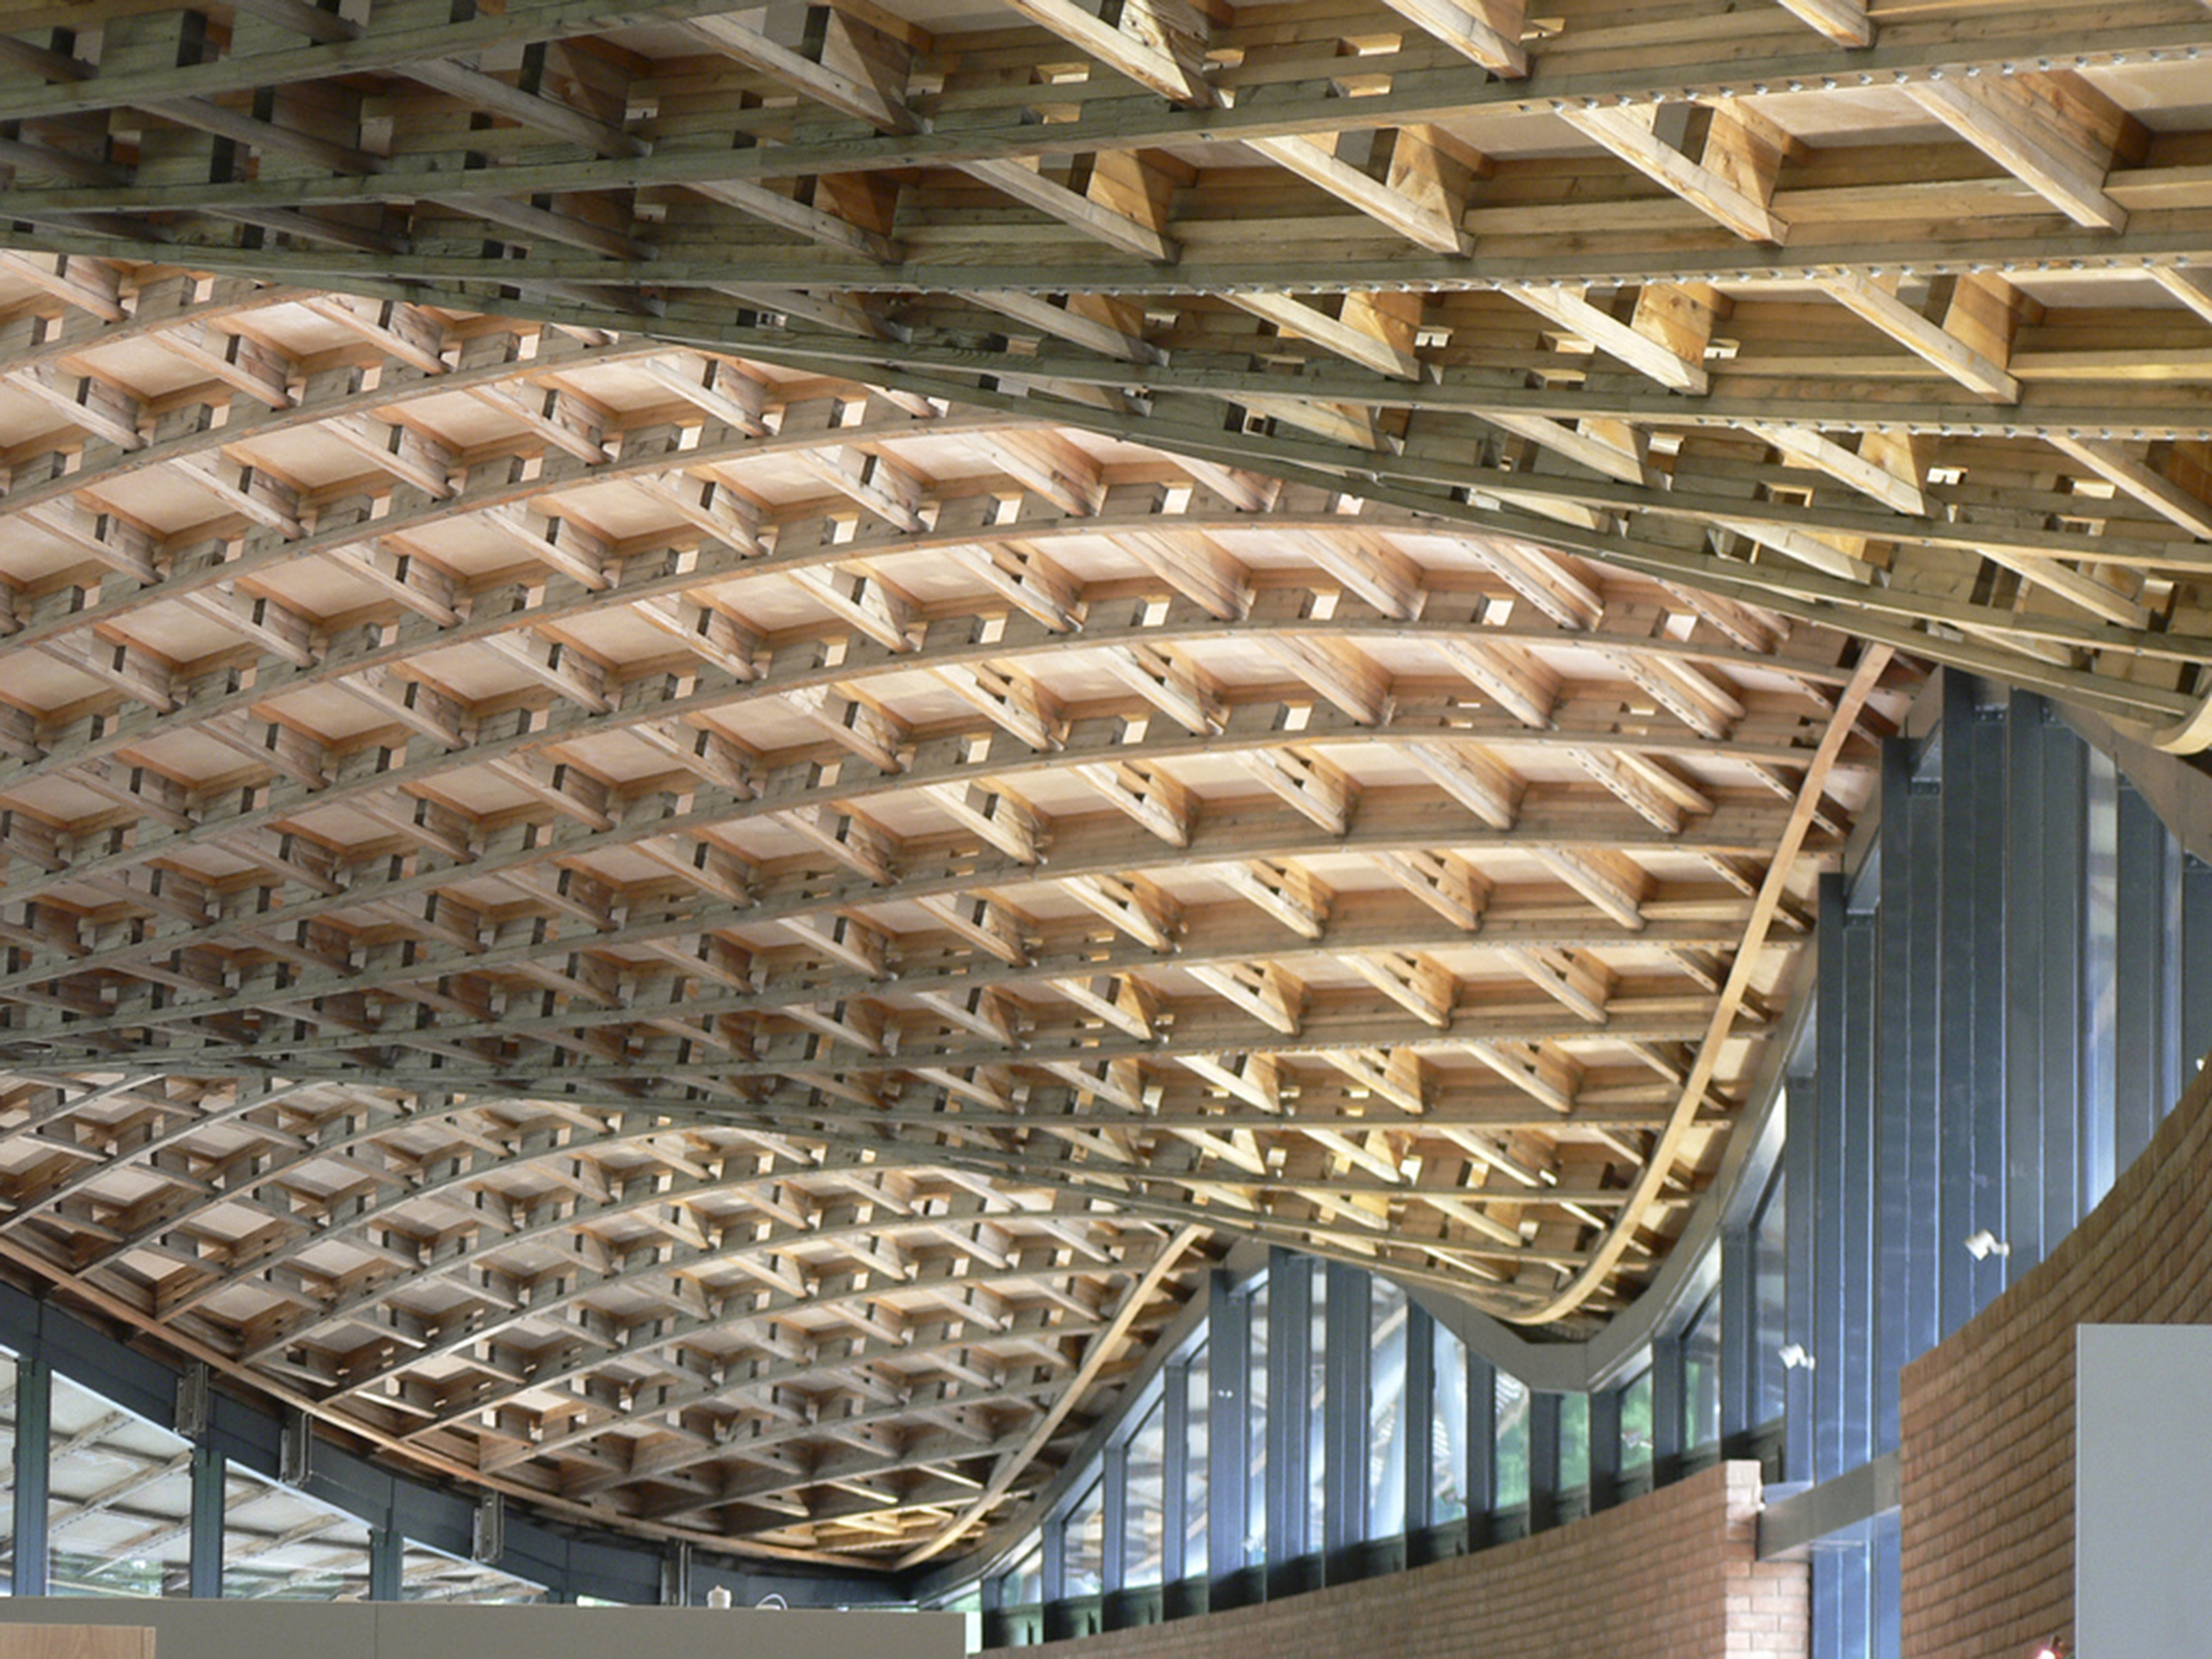
\includegraphics[width=\TwoMediaWidth]{savill_b.jpg}\label{fig:savill_a}}
%		\hspace{\MediaGutterWidth}% (%) required to prevent extra space
%		\subfloat[][Exterior view]{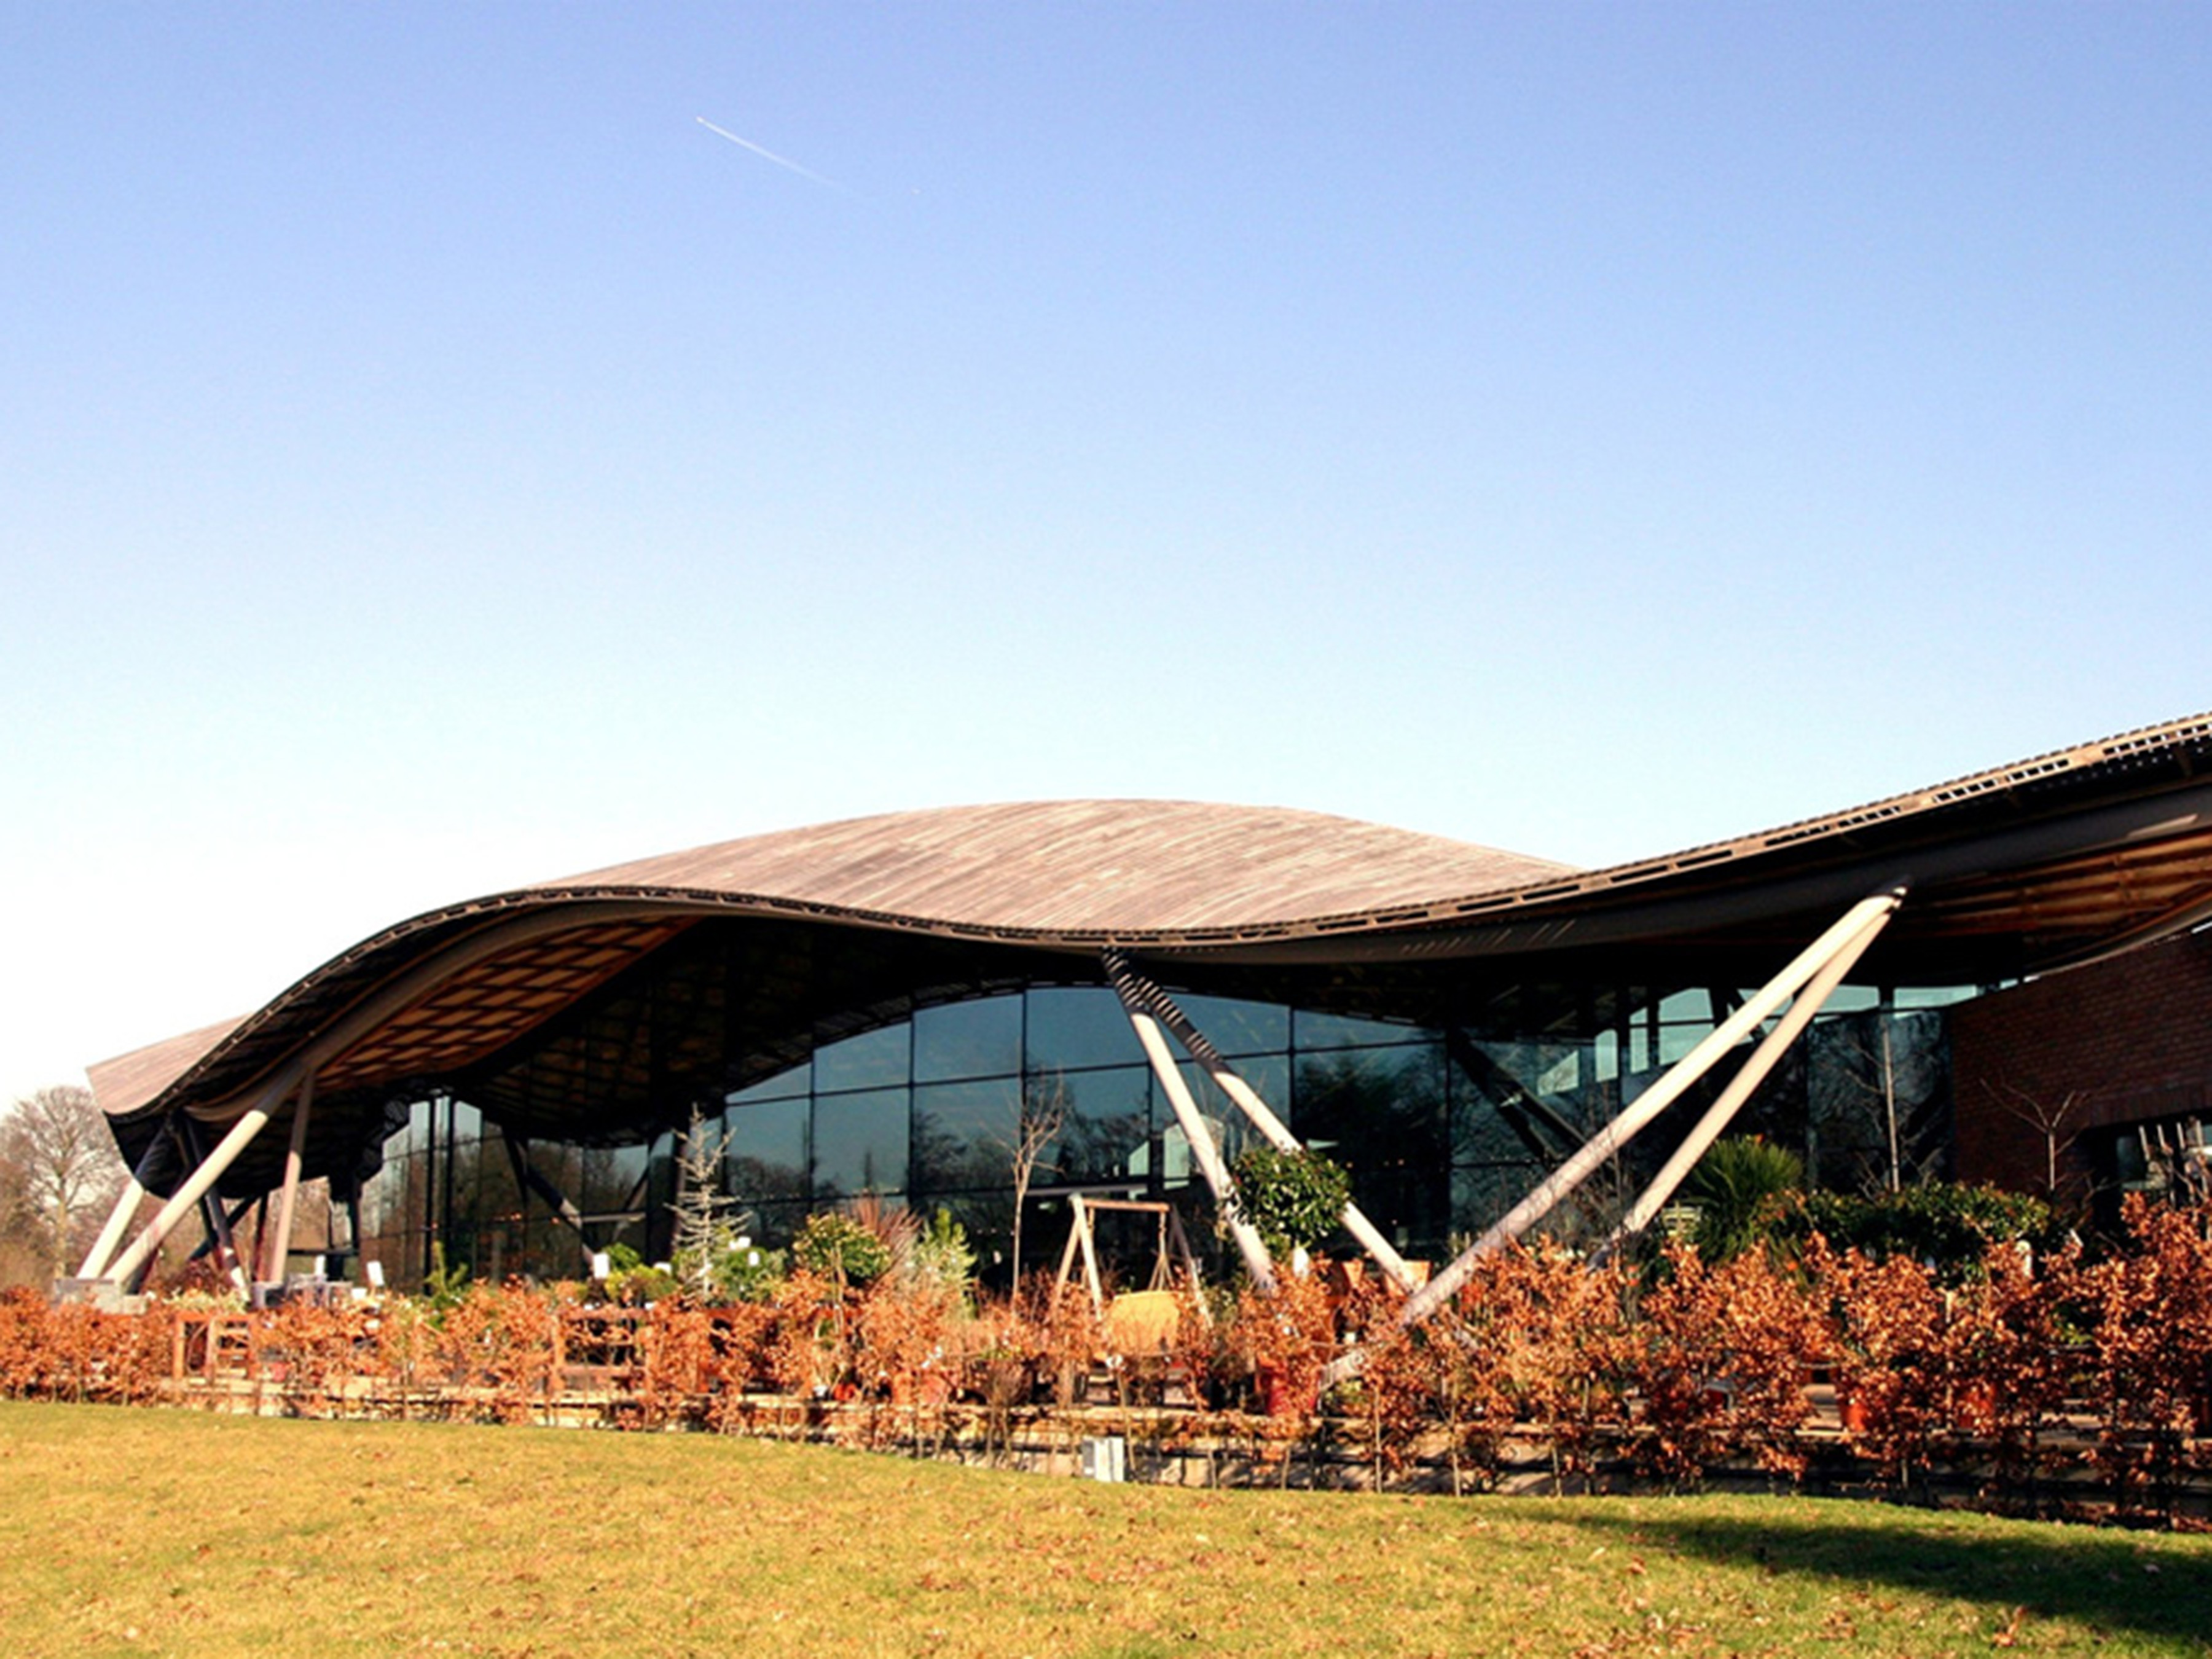
\includegraphics[width=\TwoMediaWidth]{savill_a.jpg}\label{fig:savill_b}}
%%		\vspace{10pt}
%		\captionof{figure}[Timber gridshell built in 2006 in Savill, England]{Timber gridshell built in 2006 in Savill, England.}
%		\label{fig:savill}
%%	\end{fullpage}
%\end{figure}
%%
